\input{../../../headers/dsheaders.tex}

\section*{Présentation}

Le système Skypod est une solution d'aide à la préparation de commande dans des zones de stockage de grande capacité. Il est conçu en France (région Hauts-de-France) par la société Exotec.

Sa flexibilité et son adaptabilité en font un leader de son domaine, ce qui a permis à Exotec de devenir en 2022 la première licorne industrielle française (« start-up » valorisée à plus d'un milliard de dollars US). De grands noms internationaux du commerce en ligne ou physique comptent parmi ses principaux clients.

L'une de ses spécificités est son robot manipulateur de bac qui peut évoluer dans les trois dimensions.

Il peut ainsi se déplacer sur le sol pour circuler dans les allées et rejoindre les postes de livraison figure \ref{fig01}. Mais il peut également évoluer verticalement pour atteindre les bacs dans lesquels les produits sont stockés figure \ref{fig02}.

\begin{figure}[!ht]
  \centering
  \begin{minipage}[b]{0.48\linewidth}
    \centering
    
\includegraphics[width=\linewidth]{img/fig01.png}
    \caption{Robot évoluant horizontalement}
    \label{fig01}
  \end{minipage}
  \hfill
  \begin{minipage}[b]{0.48\linewidth}
    \centering
    
\includegraphics[width=\linewidth]{img/fig02.png}
    \caption{Robot évoluant verticalement}
    \label{fig02}
  \end{minipage}
\end{figure}

Quatre composants permettent de mettre en \oe{}uvre cette solution figure \ref{fig03} :
\begin{itemize}
  \item la flotte de robots qui transporte les bacs entre opérateurs et zones de stockage ;
  \item les racks, permettant de stocker les bacs et dont le positionnement et la structure permettent
    les déplacements horizontaux et verticaux des robots ;
  \item les stations qui permettent aux opérateurs de déposer et récupérer les produits dans les bacs
    apportés par les robots ;
  \item le serveur permettant de gérer la flotte de robots en lien avec les consignes données par les
    stations.
\end{itemize}

Ce sujet s'intéresse particulièrement aux déplacements du robot. Un extrait du cahier des charges
est donné sous forme de diagramme d'exigence par la figure \ref{fig25} de l'\textbf{annexe~2}.

% Figure 3 : Diagramme de définition de blocs
\begin{figure}[!ht]
  \centering
  
\includegraphics[width=0.9\linewidth]{img/fig03.png}
  \caption{Diagramme de définition de blocs d'un robot Skypod}
  \label{fig03}
\end{figure}

% Figure 4 : Principaux composants
\begin{figure}[H]
  \centering
  
\includegraphics[width=.9\linewidth]{img/fig04.png}
  \caption{Principaux composants de la solution Skypod}
  \label{fig04}
\end{figure}

\paragraph{Analyse structurelle du robot}

La structure du robot est présentée figure \ref{fig03}. Ce robot est constitué d'un \textit{châssis} et de différents
sous-systèmes.

\begin{itemize}
  \item La \textit{partie commande} contrôle le robot, communique avec le serveur et fournit des consignes aux autres sous-systèmes,
  \item Le \textit{système de déplacement au sol} permet au robot de se déplacer au sein de l'entrepôt. Il est composé de deux roues motrices (droite et gauche) commandées par deux moteurs et de deux autres roues libres permettant de garantir une bonne stabilité au sol figure \ref{fig01},
  \item Deux \textit{systèmes de déplacement vertical} (droit et gauche) permettent au robot de s'élever entre les racks afin d'atteindre une hauteur donnée. Ils entraînent quatre pignons situés dans chaque coin du robot qui eux-même engrènent sur des chaînes tendues verticalement le long des racks figures \ref{fig02} et figure \ref{fig13}. La liaison pignon/chaîne se comporte comme une liaison pignon/crémaillère,
  \item Deux \textit{systèmes de bras rétractables} facilitent le déplacement au sol, chaque système de déplacement vertical est positionné sur un bras rétractable. Ils sont rentrés au sein du châssis lors des déplacements au sol, puis sortis lors des déplacements verticaux afin que les pignons entrent en contact avec les chaînes tendues. Un robot ne peut donc évoluer horizontalement qu'au sol,
  \item Un \textit{système de prise et dépose de bac} translate le bac de sa position de stockage dans le rack à sa position de transport sur le robot (ou inversement). Il est constitué d'une fourche télescopique qui se déploie figures \ref{fig05} et \ref{fig06} afin de se positionner sous le bac, puis rentre en déplaçant le bac avec elle.
\end{itemize}

\begin{figure}[H]
  \centering
  \begin{minipage}[b]{0.45\linewidth}
    \centering
    
\includegraphics[width=\linewidth]{img/fig05.png}
    \caption{Prise d'un bac (fourche sous le bac dans un rack)}
    \label{fig05}
  \end{minipage}
  \hfill
  \begin{minipage}[b]{0.45\linewidth}
    \centering
    
\includegraphics[width=\linewidth]{img/fig06.png}
    \caption{Fourche déployée}
    \label{fig06}
  \end{minipage}
\end{figure}



% ===========================================================
\section{Déroulement d'une préparation de commande}
% ===========================================================

\paragraph{Objectif} Étudier le comportement séquentiel du robot lors d'une préparation de commande.

Une préparation de commande se déroule en plusieurs étapes. Après réception de la demande un traitement est effectué afin d'affecter les tâches à réaliser à un ou plusieurs robots en fonction du nombre de produits demandés et à un opérateur situé sur une station. Le ou les robots vont ensuite chercher les bacs contenant les produits nécessaires à la commande et les rapportent à la station.

Enfin l'opérateur effectue la mise en carton et expédie la commande.

Le déplacement d'un robot lui permettant d'aller prendre un bac s'effectue en plusieurs phases. Le robot se déplace d'abord au sol de sa position de départ jusqu'au pied de la rangée verticale du rack qui contient le bac à prendre. Une fois en position ses bras rétractables sortent ce qui permet aux pignons motorisés d'engrener sur les chaînes tendues verticalement, générant ainsi l'ascension du
robot. Pour prendre un bac le robot s'immobilise de façon à ce que la surface de la fourche soit située 5~cm en-dessous du fond du bac. La fourche télescopique est alors sortie. Puis le robot monte de 10~cm, la fourche est ensuite rentrée afin de translater le bac sur le robot. Le robot peut désormais descendre jusqu'au sol, puis rentrer ses bras rétractables et se déplacer de nouveau au sol jusqu'à la station.

Le comportement séquentiel du robot est décrit par le diagramme d'état donné sur l'\textbf{annexe 4}. Le tableau \ref{tab01} fournit la description des ordres des moteurs et le tableau \ref{tab02} les informations reçues par la partie commande. Dans cette partie les durées des phases d'accélération et de décélération sont négligées pour tous les mouvements.


\newpage

\begin{table}[!ht]
\renewcommand{\arraystretch}{1.3}
\begin{tabular}{|p{3.3cm}|p{8cm}|p{4.5cm}|}
  \hline
  \textbf{Ordres moteurs} & \textbf{Rôle} & \textbf{Valeurs} \\
  \hline
  \multicolumn{3}{|l|}{\textit{Système de déplacement au sol :}} \\
  \hline
  M\_RoueG & Consigne de vitesse de la roue gauche & Valeurs continues \\
  M\_RoueD & Consigne de vitesse de la roue droite & entre $-V_{max}$ et $V_{max}$ \\
  \hline
  \multicolumn{3}{|l|}{\textit{Bras rétractables :}} \\
  \hline
  M\_BrasG & Déplacement du bras gauche & $0$ : pas de déplacement \\
  M\_BrasD & Déplacement du bras droit  & $+1$ : sortie des bras \\
            &                            & $-1$ : rentrée des bras \\
  \hline
  \multicolumn{3}{|l|}{\textit{Système de déplacement vertical :}} \\
  \hline
  M\_PignonG & Consignes de vitesse des pignons gauches & $GV$ : grande vitesse \\
  M\_PignonD & Consignes de vitesse des pignons droits  & $PV$ : petite vitesse \\
             &                                           & $-GV$, $-PV$ : descente \\
             &                                           & $+GV$, $+PV$ : montée \\
  \hline
  \multicolumn{3}{|l|}{\textit{Fourche télescopique :}} \\
  \hline
  M\_Fourche & Déplacement de la fourche & $0$ : pas de déplacement \\
             &                           & $+1$ : sortie de la fourche \\
             &                           & $-1$ : rentrée fourche \\
  \hline
\end{tabular}
\caption{\label{tab01}Variables de sortie de la partie commande}
\end{table}

\begin{table}[!ht]
\renewcommand{\arraystretch}{1.3}
\begin{tabular}{|p{7cm}|p{9cm}|}
  \hline
  \textbf{Informations} & \textbf{Rôle} \\
  \hline
  \multicolumn{2}{|l|}{\textit{Capteurs fin de course (détecteur) :}} \\
  \multicolumn{2}{|l|}{Leur sortie vaut 1 si la position détectée est atteinte ; 0 sinon} \\
  \hline
  BrasG\_sorti et BrasG\_rentré & Capteurs du bras rétractable gauche \\
  BrasD\_sorti et BrasD\_rentré & Capteurs du bras rétractable droit \\
  Fourche\_sortie et Fourche\_rentrée & Capteurs de la fourche \\
  \hline
  \multicolumn{2}{|l|}{\textit{Position courante du robot :}} \\
  \hline
  alt\_courante & position verticale du robot \\
  pos\_courante & position au sol du robot \\
  \hline
  \multicolumn{2}{|l|}{\textit{Position à atteindre :}} \\
  \hline
  bac & $bac = +1 \to$ prise de bac ; présence de bac sur le robot -- mission de prise ou de dépose de bac \\
  pos\_finale & position au sol d'arrivée \\
  etag & numéro d'étagère ($\times 40$~mm : étagère du bas) où se situe le bac à prendre \\
  \hline
\end{tabular}
\caption{\label{tab02}Variables d'entrée de la partie commande}
\end{table}

On s'intéresse au scénario d'un robot allant chercher un bac sur l'étagère~4 ($etag = 4$). On notera que la distance verticale entre deux étagères est de 40~cm. Pour ce scénario le temps est discrétisé $t_0, t_1, \ldots, t_{k-1}, t_k, t_{k+1}, \ldots$ pour $k \in \mathbb{N}$ avec un pas de temps $t_{k+1} - t_k = \Delta t$ constant. On notera les constantes
suivantes :

\begin{center}
\begin{tabular}{ll}
  Temps de rentrée/sortie de la fourche : & $2\Delta t$ \\
  Temps de rentrée/sortie des bras rétractables : & $2\Delta t$ \\
  Valeurs de consigne pour le déplacement vertical : & $dv = 5/\Delta t$~cm\,s$^{-1}$ et $pv = \frac{1}{2}dv$ \\
\end{tabular}
\end{center}

\question{Compléter le chronogramme sur le document réponse DR\ref{DR1} en suivant le scénario suivant :
\begin{itemize}
  \item à $t_0$ le robot reçoit une nouvelle destination, \texttt{pos\_finale} et \texttt{etag} sont connus ;
  \item à $t_1$ le calcul de l'itinéraire est fini et le robot commence à se déplacer vers sa destination
    \texttt{pos\_finale}, sa trajectoire est en ligne droite : M\_RoueG = M\_RoueD et la consigne est
    de $V_{max}$ ;
  \item à $t_3$ le robot arrive à \texttt{pos\_finale} et commence à sortir les bras ;
  \item le robot monte et récupère le bac puis redescend au sol ;
  \item une fois au sol le robot retourne à sa position de départ, consigne de $-V_{max}$.
\end{itemize}}

% ===========================================================
\section{Trajectoire du robot en phase de déplacement au sol}
% ===========================================================

\paragraph{Objectif} Étudier le comportement cinématique du robot en phase de déplacement au sol.
 
Pour ses déplacements au sol le robot possède deux roues motrices~2 et~3 insérées dans deux chaînes de puissance différentes et donc entraînées par deux moteurs différents. Pour assurer la stabilité au sol deux autres roues laissées libres de leurs mouvements, dites \og folles \fg, sont associées à un mécanisme permettant aux quatre roues d'être en contact avec le sol en permanence.

On s'intéresse à une trajectoire composée d'un segment droit, d'une courbe permettant au robot de tourner d'un quart de tour vers la gauche, puis d'un dernier segment droit figure \ref{fig07}.

% Figure 7 : Trajectoire globale (non représentée ici, à insérer)
% Figure 8 : Paramétrage du robot au sol
\begin{figure}[H]
  \centering
  \begin{minipage}[b]{0.47\linewidth}
    \centering
    
\includegraphics[width=\linewidth]{img/fig07.png}
    \caption{Paramétrage du robot au sol}
    \label{fig07}
  \end{minipage}
  \hfill
  \begin{minipage}[b]{0.47\linewidth}
    \centering
    
\includegraphics[width=\linewidth]{img/fig08.png}
    \caption{Paramétrage de la roue~2 en contact avec le sol en I}
    \label{fig08}
  \end{minipage}
\end{figure}

Le robot est vu comme un ensemble de trois solides : le châssis~1, la roue gauche~2 en contact avec
le sol~0 au point~$I$ et la roue droite~3 en contact avec le sol~0 au point~$J$.

Les roues~2 et~3 sont en liaison pivot d'axe respectivement $(A,\vec{z}_1)$ et $(B,\vec{z}_1)$ avec le châssis~1 et on
considérera qu'il y a roulement sans glissement de la roue~2 (respectivement roue~3) par rapport au
sol~0 en~$I$ (respectivement en~$J$). Pour des raisons de simplification les roues « folles » ne sont pas
étudiées ou représentées mais imposent que le châssis~1 ne peut être en rotation que selon $\vec{y}_1$.

On définit :
\begin{itemize}
  \item $R_0(O_0,\vec{x}_0,\vec{y}_0,\vec{z}_0)$ le référentiel supposé galiléen lié au sol~0. On notera que $\vec{y}_0$ est donc la verticale
    ascendante.
  \item $R_1(O_1,\vec{x}_1,\vec{y}_1,\vec{z}_1)$ le référentiel lié au châssis~1 avec $\theta_{10} = \widehat{(\vec{z}_0,\vec{z}_1)} = \widehat{(\vec{x}_0,\vec{x}_1)}$, \linebreak
  $\omega_{10}(t)~=~\dfrac{\mathrm{d}\theta_{10}(t)}{\mathrm{d}t}$ et la vitesse du robot $\vec{V}(O_1 \in 1/0) = V(t)\cdot\vec{x}_1$.
  \item $R_2(A,\vec{x}_2,\vec{y}_2,\vec{z}_2)$ le référentiel lié à la roue gauche~2 avec $A$ le centre de la roue, \linebreak
    $R~=~20$~mm son rayon, $\theta_{21}(t) = \widehat{(\vec{x}_1,\vec{x}_2)} = \widehat{(\vec{y}_1,\vec{y}_2)}$ et $\omega_{21}(t) = \dfrac{\mathrm{d}\theta_{21}(t)}{\mathrm{d}t}$ (figure~9).
  \item $R_3(B,\vec{x}_3,\vec{y}_3,\vec{z}_3)$ le référentiel lié à la roue droite~3 avec $B$ le centre de la roue, \linebreak
    $R~=~20$~mm son rayon, $\theta_{31}(t) = \widehat{(\vec{x}_1,\vec{x}_3)} = \widehat{(\vec{y}_1,\vec{y}_3)}$ et $\omega_{31}(t) = \dfrac{\mathrm{d}\theta_{31}(t)}{\mathrm{d}t}$ (paramétrage analogue à la roue~2).
  \item $L$ la largeur du robot : $\vv{AO_1} = \vv{O_1B} = \dfrac{L}{2}\cdot\vec{z}_1$.
\end{itemize}

\medskip

\question{À l'aide de la condition de roulement sans glissement en~$I$, donner la relation entre $V(t)$, $\omega_{21}(t)$
et $\omega_{10}(t)$.}

\question{Par un raisonnement analogue, donner directement la relation entre $V(t)$, $\omega_{31}(t)$ et $\omega_{10}(t)$.}

\question{En déduire $\omega_{10}(t)$ en fonction de $\omega_{21}(t)$ et de $\omega_{31}(t)$.}

\medskip

On s'intéresse dans un premier temps à une trajectoire rectiligne. On note $\omega_{moy}(t)$ la vitesse de rotation
des roues pour cette trajectoire, pour une vitesse $V(t) = 2m\cdot s^{-1}$.

\question{Démontrer que pour une trajectoire rectiligne $\omega_{21}(t) = \omega_{31}(t) = \omega_{moy}(t)$ et donner sa valeur.}

\medskip

On s'intéresse dans un deuxième temps à la réalisation du virage de $90^\circ$ vers la gauche (figure~\ref{fig07}).
Pour cela on fait varier la vitesse $\omega_{21}$ par une loi en trapèze et la vitesse $\omega_{31}$ par une seconde loi en
trapèze telle que $\dot{\omega}_{21}(t) = -\dot{\omega}_{31}(t)$ avec $\dot{\omega}_{21}$ et $\dot{\omega}_{31}$ les accélérations angulaires des roues~2 et~3 par
rapport au châssis.

\question{Donner dans ces conditions la valeur de l'accélération angulaire $\dot{\omega}_{10}(t)$ en fonction de $\dot{\omega}_{21}(t)$.}

\medskip

Ces lois de commande de vitesse des roues aboutissent à l'évolution de $\omega_{10}(t)$ au cours d'un virage de $90^\circ$ donnée figure~\ref{fig09}. La norme de l'accélération angulaire pendant les phases~1 et~3 est constante et notée $\gamma_{10}$.

\begin{figure}[H]
  \centering
  
\includegraphics[width=0.8\linewidth]{img/fig09.png}
  \caption{Évolution de $\omega_{10}$ lors d'un virage de $90^\circ$}
  \label{fig09}
\end{figure}

\question{En faisant l'hypothèse que $t_1 = 0$, donner les expressions littérales de $t_2$, de $t_3$ et de $t_4$ en fonction de $\omega_{10max}$ et de $\gamma_{10}$.}

\medskip

On propose plusieurs simulations de trajectoire pour différentes valeurs de $\omega_{10max}$ dont le point de
départ est de coordonnées $(0,0)$ (figure~\ref{fig10}). À des fins de comparaison la figure~\ref{fig11} présente ces trajectoires en version normalisée (point de départ et d'arrivée de coordonnées $(0,0)$ et $(1,1)$).

\question{À l'aide des figures~\ref{fig10} et \ref{fig11}, commenter l'influence de $\omega_{10max}$ sur la trajectoire du robot lors d'un virage.}

\begin{figure}[H]
  \centering
  \begin{minipage}[b]{0.47\linewidth}
    \centering
    
\includegraphics[width=\linewidth]{img/fig10.png}
    \caption{Trajectoires selon plusieurs valeurs de $\omega_{10max}$}
    \label{fig10}
  \end{minipage}
  \hfill
  \begin{minipage}[b]{0.47\linewidth}
    \centering
    
\includegraphics[width=\linewidth]{img/fig11.png}
    \caption{Trajectoires normalisées selon plusieurs valeurs de $\omega_{10max}$}
    \label{fig11}
  \end{minipage}
\end{figure}

% ===========================================================
\section{Sollicitation du robot en mouvement vertical}
% ===========================================================

%\paragraph{Objectif} Déterminer la puissance des moteurs nécessaire pour assurer le mouvement vertical du robot.

\paragraph{Objectif} Concevoir la carte d'alimentation des moteurs.

Une fois le robot positionné aux pieds des racks, les bras rétractables sont déployés afin de mettre en contact les pignons sur les chaînes tendues le long des poteaux constituant les racks. La rotation des pignons entraînera alors l'ascension du robot, figure~\ref{fig12} et \ref{fig13}.

\begin{figure}[H]
  \centering
  \begin{minipage}[b]{0.45\linewidth}
    \centering
    
\includegraphics[width=\linewidth]{img/fig12.png}
    \caption{Détail de l'engrènement d'un pignon sur la chaîne}
    \label{fig12}
  \end{minipage}
  \hfill
  \begin{minipage}[b]{0.45\linewidth}
    \centering
    
\includegraphics[width=\linewidth]{img/fig13.png}
    \caption{Vue du robot en montée (sans charge ni bac), avec pignons et chaînes redessinés}
    \label{fig13}
  \end{minipage}
\end{figure}

La structure de la chaîne de puissance permettant l'ascension du robot est schématisée figure~\ref{fig14}.

Elle est composée de deux ensembles similaires, chacun étant constitué d'un moteur d'ascension et d'un système poulie-courroie dont la poulie motrice est liée à l'arbre de sortie du moteur et la poulie réceptrice à un arbre de transmission. Ce dernier supporte également les deux pignons qui engrènent sur les chaînes tendues. La rotation des pignons va donc permettre de générer le mouvement vertical du robot. Un système annexe (non étudié ni représenté ici) permet de s'assurer que les pignons soient toujours en prise dans les chaînes.

\begin{figure}[!ht]
  \centering
  
\includegraphics[width=0.7\linewidth]{img/fig14.png}
  \caption{\label{fig14}Schématisation de la chaîne de puissance associée à l'ascension du robot. Vue de dessus du robot, pesanteur selon $-\vec{y}_0$.}
\end{figure}

\subsection{Hypothèses et paramétrage}

\begin{itemize}
  \item On note $R_0(O_0,\vec{x}_0,\vec{y}_0,\vec{z}_0)$ le référentiel supposé galiléen lié au sol,
  \item On note $S$ l'ensemble des pièces en mouvement : S = \{\text{Châssis} + \text{Moteurs} \linebreak + \text{Systèmes Poulie-Courroie} + \text{Arbres transmission} + \text{Pignons} + \text{Bac rempli}\} de masse $m_S$ et de centre d'inertie $G_S$ tel que $\vv{OG_S} = x_{G_S}\cdot\vec{x}_0 + y_{G_S}(t)\cdot\vec{y}_0 + z_{G_S}\cdot\vec{z}_0$.
  \item La position du centre de gravité n'est pas le centre géométrique du robot car la masse transportée est potentiellement excentrée.
  \item Le mouvement du châssis~1 par rapport au sol~0 est une translation de vitesse \\ $v_a(t)\cdot\vec{y}_0=\dot{y}_{G_S}(t)\cdot\vec{y}_0$.
    Ainsi $v_a(t)$ est la vitesse d'ascension du robot.
  \item On définit les vitesses de rotation du moteur~4 et de l'arbre de transmission~5 par rapport au
    châssis~1 par respectivement $\vec{\Omega}_{m/1} = \omega_{m1}(t)\cdot\vec{z}_0$ et $\vec{\Omega}_{5/1} = \omega_{51}(t)\cdot\vec{z}_0$. Les vitesses de rotation du
    moteur~4$'$ $\vec{\Omega}_{m'/1} = \omega_{m'1}(t)\cdot\vec{z}_0$ et de l'arbre de transmission~5$'$ $\vec{\Omega}_{5'/1} = \omega_{5'1}(t)\cdot\vec{z}_0$ sont opposées respectivement à celles de~4 et de~5.
%  \item L'action mécanique du moteur~4 est modélisée par un torseur couple dont le moment sur son axe de rotation vaut $C_m(t)$. On suppose ici que les deux moteurs délivrent le même couple mais en sens opposés.
%  \item Les différents frottements internes et externes sont ramenés sur l'axe de rotation de chaque arbre de transmission et sont modélisés par un moment constant $C_f\cdot\vec{z}_0$ sur l'arbre~5, $C'_f\cdot\vec{z}_0$ sur l'arbre~5$'$. Ces deux couples sont opposés aux vitesses de rotation des arbres~5 et~5$'$ de sorte que la valeur numérique de $C_f$ est de signe opposé à celui de $\omega_{51}(t)$ et que la valeur numérique de $C'_f$ est de signe opposé à celui de $\omega_{5'1}(t)$.
  \item On note respectivement $R_m$, $R_r$ et $R_p$ les rayons d'enroulement des poulies motrices et réceptrices et le rayon primitif des pignons.
%  \item On note respectivement $J_m$ et $J_5$ les moments d'inertie selon leurs axes de rotation d'un arbre moteur (poulie comprise) et d'un arbre de transmission (poulie et roues dentées comprises).
  \item L'attraction de pesanteur est portée par $-\vec{y}_0$ de sorte que $\vec{g} = -g\cdot\vec{y}_0$.
%  \item L'inertie de la courroie est négligée.
  \item Le châssis inclut la batterie, les cartes électroniques et la connectique.
\end{itemize}

%\question{Déterminer l'expression de l'énergie cinétique $E_c(S/R_0)$ de l'ensemble $S$ par rapport au repère $R_0$.}
%
%~\
%
La liaison entre un pignon et une chaîne correspond à un roulement sans glissement sur le rayon primitif $R_p$ du pignon.

\question{Exprimer le vecteur de la vitesse d'ascension du robot $v_a(t)\cdot\vec{y}_0$ en fonction de la vitesse de rotation de l'arbre moteur $\omega_{m1}(t)$.}

%\question{En déduire l'expression de l'inertie équivalente notée $J_{eq}$ de l'ensemble $S$ rapportée à l'arbre moteur, en fonction de $m_s$, $J_m$, $J_5$ et des grandeurs géométriques.}
%
%\question{Déterminer l'expression de la somme des puissances extérieures (galiléennes) et intérieures à l'ensemble $S$. On ne fera apparaître que $\omega_{m1}(t)$ comme variable cinématique.}
%
%\question{Déduire des questions précédentes, en justifiant rigoureusement, l'expression du couple moteur $C_m(t)$ en fonction de $\dot{\omega}_{m1}(t)$ et des grandeurs caractéristiques constantes du système.}
%
%\medskip
%
%On donne figure~\ref{fig15} le profil de vitesse choisi pour l'évolution de la vitesse verticale du robot pour un cycle de montée/descente et dans le tableau \ref{tab03} les valeurs numériques associées. On souhaite
%déterminer l'évolution correspondante du couple moteur.
%
%\begin{figure}[H]
%  \centering
%  
\includegraphics[width=0.7\linewidth]{img/fig15.png}
%  \caption{Pilotage adopté pour la vitesse d'ascension pour un cycle de montée/descente}
%  \label{fig15}
%\end{figure}

\begin{table}[!ht]
\begin{center}
\renewcommand{\arraystretch}{1.3}
\begin{tabular}{|ll|ll|}
  \hline
  \multicolumn{4}{|l|}{\textbf{Données}} \\
  \hline
  $R_m = 20~mm$         & & $t_1 = 2$~s & \\
  $R_r = 30~mm$         & & $t_2 = 8$~s & \\
  $|C_f| = |C'_f| = 1~N\cdot m$   & & $t_3 = 10$~s & \\
  $J_{eq} = 1{,}14 \times 10^{-1}~kg\cdot m^2$ & & $t_4 = 12$~s  & \\
  $R_p = 38~mm$                & &  $t_5 = 18$~s & \\
  $v_{max} = 2~m\cdot s^{-1}$   & & $t_f = 20$~s & \\
  $m_s = 78~kg$                & & & \\
  $K_c=1~N\cdot m\cdot A^{-1}$ & & & \\
  $R_m=3\Omega$ & & & \\
  $U_{alim}=48V$ & & & \\
  \hline
\end{tabular}
\end{center}
\caption{\label{tab03}Valeurs numériques utiles}
\end{table}

%\medskip
%
%\question{Compléter le DR\ref{DR2} en traçant l'évolution de l'accélération angulaire $\dot{\omega}_{m1}(t)$ au cours du temps.}
%
%\question{Tracer sur le DR\ref{DR3} l'évolution de $C_f$ au cours du temps.}
%
%\medskip
%
%Il est alors possible, grâce aux travaux précédents, de calculer l'évolution du couple moteur $C_m(t)$ pour les différentes phases tableau~\ref{tab04}.
%
%\begin{table}[!ht]
%\renewcommand{\arraystretch}{1.3}
%\begin{tabular}{|l|c|c|c|c|c|c|}
%  \hline
%  intervalle & de 0 à $t_1$ & de $t_1$ à $t_2$ & de $t_2$ à $t_3$ & de $t_3$ à $t_4$ & de $t_4$ à $t_5$ & de $t_5$ à $t_f$ \\
%  \hline
%  $C_m(t)$ & $-17~N\cdot m$ & $-15{,}5~N\cdot m$ & $-14~N\cdot m$ & $-12~N\cdot m$ & $-13{,}5~N\cdot m$ & $-15~N\cdot m$ \\
%  \hline
%\end{tabular}
%\caption{\label{tab04}Évolution de $C_m(t)$ au cours du temps}
%\end{table}
%
%\medskip
%
%D'après les exigences, le moteur envisagé pour la motorisation est capable de fournir une puissance mécanique de 1\,000~W.
%
%\question{Après avoir précisé l'instant correspondant, déterminer la valeur numérique de la puissance maximale que le moteur devra développer pour assurer le mouvement étudié. Conclure quant au choix du moteur envisagé.}

\subsection{Détermination de l'architecture du pré-actionneur électrique des moteurs à courant continu}

On considère que les 2 moteurs à courant continu ainsi que les 2 circuits électriques sont identiques et que ces derniers sont soumis à la même tension d'alimentation constante $U_{alim}$. Afin de faire varier la tension d'alimentation d'un moteur, on utilise un hacheur, placé en amont de chaque moteur. On se propose ici de déterminer la structure du hacheur compatible avec les éventuels différents modes de fonctionnement des moteurs lors d'un scan.

\subsubsection{Analyse de la pertinence d'un hacheur simple série}

On considère dans un premier temps un hacheur simple série figure \ref{td02_07} constitué d'un interrupteur commandé de type \og Transistor bipolaire à grille isolée (IGBT) \fg, de fréquence de découpage très grande par rapport au temps caractéristique électrique du circuit, et d'une diode. L'interrupteur $K_1$ et la diode D sont supposés parfaits.

\begin{figure}[!ht]
 \centering 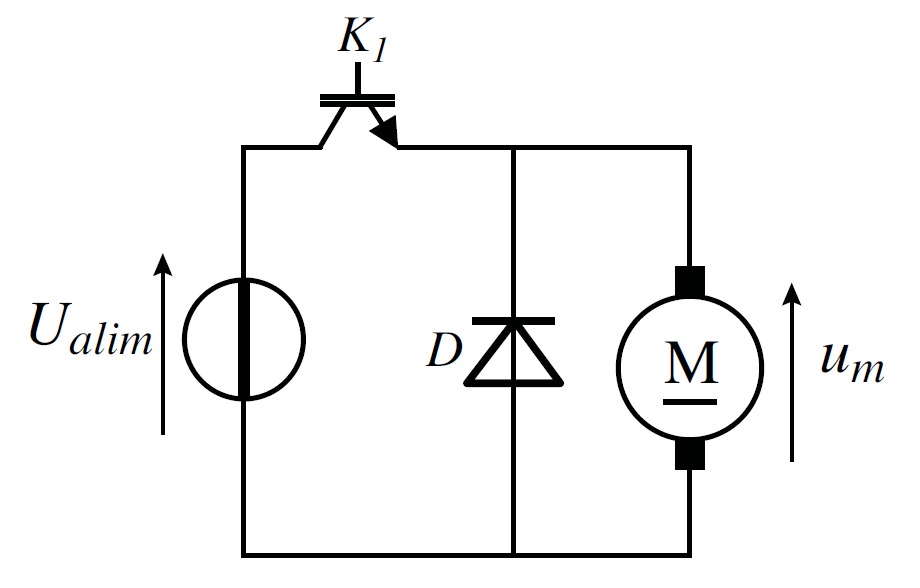
\includegraphics[width=0.4\linewidth]{img/td02_07}
 \caption{Schéma électrique de l'architecture simplifiée d'un hacheur simple série}
 \label{td02_07}
\end{figure}

\question{En considérant la phase de montée à vitesse constante, préciser sur le document réponse, en couleur, les mailles dans lesquelles le courant circule lorsque le transistor est bloqué (rouge) ou passant (bleu). Ce type de hacheur permet-il les deux sens de courant dans le moteur (expliquer en trois lignes maximum). Préciser alors, sur le document réponse, le(s) quadrant(s) dans le(s)quel(s) le moteur à courant continu peut fonctionner avec ce hacheur.}

~\

On considère maintenant la phase de descente. Lors de cette phase, les moteurs doivent tourner dans le sens inverse de celui de la phase de montée.

\question{Le hacheur proposé permet-il ces deux modes de fonctionnement ?}

\subsubsection{Analyse de la pertinence d'un hacheur réversible en tension}

En considère maintenant un hacheur réversible en tension dont le schéma d'une structure simplifiée est donné sur la figure \ref{td02_08}. Sur une période de découpage T, les interrupteurs sont pilotés de la manière suivante ($\alpha$ étant le rapport cyclique compris entre 0 et 1) :
\begin{itemize}
 \item sur l'intervalle $[0,\alpha T[$ les interrupteurs $K_1$ sont passants,
 \item sur l'intervalle $[\alpha T , T[$ les interrupteurs $K_1$ sont bloqués.
\end{itemize}

\begin{figure}[!ht]
 \centering 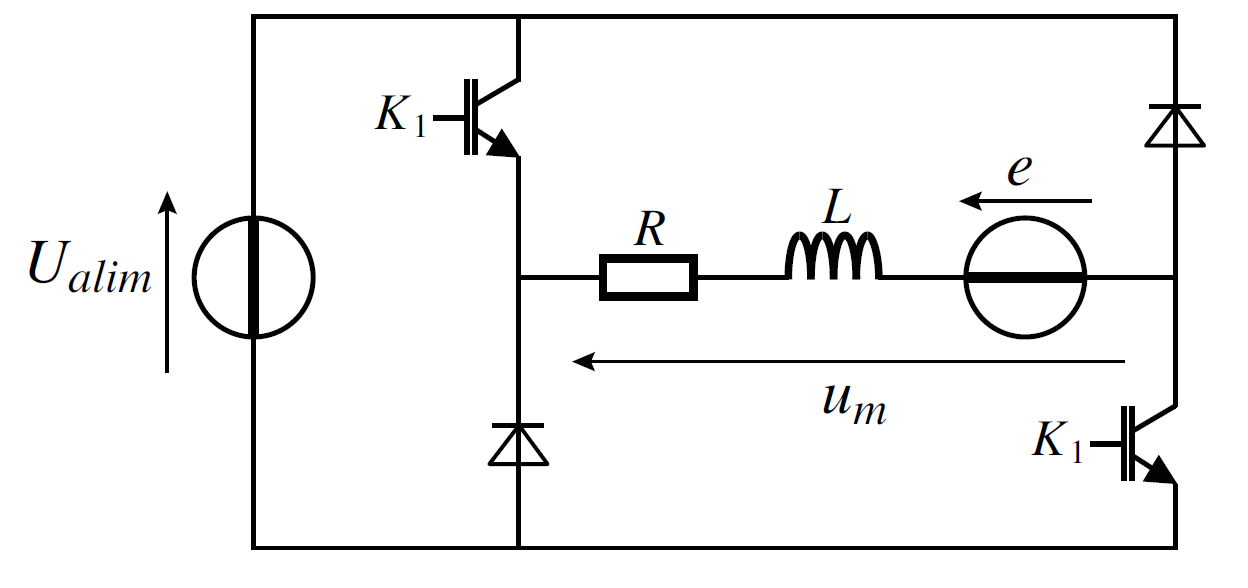
\includegraphics[width=0.7\linewidth]{img/td02_08}
 \caption{Schéma électrique de l'architecture simplifiée d'un hacheur réversible en tension}
 \label{td02_08}
\end{figure}

\question{En considérant la tension $U_{alim}$ constante, représenter sur le chronogramme du document réponse le graphe de $u_m(t)$ sur une période $T$. Déterminer l'expression de la valeur moyenne de $u_m(t)$ sur une période $T$ (notée $<u_m>$) en fonction de $U_{alim}$ et de $\alpha$. Quelle est la plage de variation de $<u_m>$ ? Cette plage est-elle compatible avec les deux sens de rotation ?}

\question{Préciser sur la figure du document réponse le(s) quadrant(s) dans le(s)quel(s) le moteur à courant continu peut fonctionner avec ce hacheur. Ce hacheur est-il compatible avec tous les modes de fonctionnements abordés (en phase de montée et en phase de descente) ?}

\subsubsection{Analyse de l'influence du hacheur sur l'évolution du courant dans le circuit}

Quels que soient les résultats obtenus précédemment, on considère pour la suite le hacheur réversible en tension. Dans le cas où cette architecture ne serait pas compatible avec tous les modes de fonctionnement des moteurs, un hacheur réversible en courant et tension serait adopté. Ces deux architectures ayant le même impact sur la forme du courant dans le circuit au cours du temps, on se contente ici d'analyser le comportement du circuit avec un hacheur réversible en tension.

On considère la phase de montée à vitesse constante et le rendement de la chaîne de transmission de puissance est pris égal à 1, soit $C_f=C'_f=0$.

On donne le bilan des puissances suivant: $2\cdot C_m\cdot\omega_{m1}(t)=m_S\cdot g\cdot v_a(t)$.

%Avec:
%\begin{itemize}
% \item Rayon du pignon (mm): $p_v=10$,
% \item Rapport de réduction : $N=5$,
% \item Masse(kg): $M=400$,
% \item Constante de couple (N.m/A): $K_i=0,12$,
% \item Résistance ($\Omega$): $R=2$,
% \item Tension d'alimentation (V): $U_{alim}=48$.
%\end{itemize}

\question{Déterminer la valeur du courant $i_m(t)$ traversant chaque moteur.}

~\

On cherche maintenant à déterminer l'évolution du courant pendant cette phase sur une période T. Sur l'intervalle de temps $[0,\alpha T[$, les transistors $K_1$ sont passants, figure \ref{td02_08}. L'intensité du courant à $t = 0$, est notée $i_0$.

\question{Déterminer l'équation différentielle pilotant le comportement temporel de l'intensité du courant $i_m(t)$ traversant le moteur.}

\question{Expliquer pourquoi $e(t)$ peut être considérée par hypothèse comme constante (on notera sa valeur $e_m$) puis, par la méthode de votre choix, déterminer l'expression de la fonction $i_m(t)$ en fonction de : $U_{alim}$, $e_m$, $R$, $i_0$ et une constante de temps $\tau_e=\frac{L}{R}$.}

\question{On suppose que $T<<\tau_e$. En faisant un développement limité à l'ordre 1 de $i_m(t)$ au voisinage de zéro, déterminer $i(\alpha.T)$. Tracer sur la figure du document réponse l'allure du graphe de $i_m(t)$ sur une période complète $[0, T]$.}

\question{En considérant toujours $T << \tau_e$, déterminer l'expression de l'augmentation de courant sur l'intervalle $[0, \alpha T[$: $\Delta i =i(\alpha T)-i_0$  en fonction de $U_{alim}$, $e_m$, $R$, $\tau_e$, $T$ et $\alpha$.}

~\

Afin que cette évolution de l'intensité du courant sur une période T ne perturbe pas le comportement mécanique du moteur, on impose que $\Delta_i \simeq \frac{i_0}{100}$.

\question{En déduire une condition sur l'ordre de grandeur de $T$ par rapport à $\tau_e$. On prendra $e_m=36V$ pour l'application numérique.}

% ===========================================================
\section{Asservissement de l'assiette du robot}
% ===========================================================

 \paragraph{Objectif} Modéliser et mettre au point l'asservissement de l'inclinaison du robot.
 
Cette partie s'intéresse au contrôle de l'inclinaison du robot lors de la phase d'ascension repérée par son angle d'inclinaison par rapport à l'horizontale noté $\alpha(t)$ (aucune rapport avec le $\alpha$ de la partie III). Cette phase est schématisée figure~\ref{fig16}, dans le cas horizontal ($\alpha = 0$) et dans le cas incliné ($\alpha \ne 0$). Les pignons sont ramenés dans le plan médian. Pour rappel un sous-système non étudié ici permet de garantir le contact pignon/chaîne.

\begin{figure}[H]
  \centering
  
\includegraphics[width=0.9\linewidth]{img/fig16.png}
  \caption{Schématisation du robot en phase d'ascension, dans la configuration horizontale (à
    gauche) et inclinée (à droite).}
  \label{fig16}
\end{figure}

On présente figure~\ref{fig17} la structure générale de l'asservissement associée à la phase étudiée. Cette inclinaison est modifiée grâce au différentiel de vitesse et de position des pignons gauche et droit. Un inclinomètre mesurant l'inclinaison du robot permet au calculateur de gérer l'asservissement.

\begin{figure}[H]
  \centering
  
\includegraphics[width=0.8\linewidth]{img/fig17.png}
  \caption{Structure générale de l'asservissement en inclinaison du robot en phase d'ascension.}
  \label{fig17}
\end{figure}

\subsection{Modélisation de la motorisation}

Un moteur d'ascension peut se modéliser comme une machine à courant continu dont on rappelle les équations :
\begin{eqnarray}
  u_m(t) = e(t) + R_m\cdot i_m(t) + L_m\cdot \frac{\mathrm{d}i_m(t)}{\mathrm{d}t} \nonumber\\
  e(t) = K_e\cdot \omega_{m1}(t) \nonumber\\
  C_m(t) = K_c\cdot i_m(t) \nonumber\\
  J_{eq}\cdot \frac{\mathrm{d}\omega_{m1}(t)}{\mathrm{d}t} = C_m(t) - C_r - C_f(t)\nonumber
\end{eqnarray}

et dont les notations sont détaillées tableau~\ref{tab05}. Le schéma-blocs correspondant est ébauché dans le DR. Les notations des variables dans le domaine de Laplace sont répertoriées dans le tableau~\ref{tab06}.

\medskip

\begin{table}[!ht!]
\renewcommand{\arraystretch}{1.3}
\begin{tabular}{|p{7.5cm}|p{8.5cm}|}
  \hline
  \textbf{Variables} & \textbf{Constantes} \\
  \hline
  $u_m(t)$ : tension moteur (V) & $R_m = 3\ \Omega$ : résistance de l'induit \\
  $i_m(t)$ : intensité moteur (A) & $L_m = 1$~mH : inductance de l'induit \\
  $e(t)$ : force contre-électromotrice (V) & $K_c = 1~N\cdot m\cdot A^{-1}$ : constante de couple \\
  $C_m(t)$ : couple électromagnétique ($N\cdot m$) & $K_e = 1~V\cdot s\cdot rad^{-1}$ : constante électrique \\
  $C_r$ : couple résistant dû à la pesanteur & $J_{eq} = 1,14 \times 10^{-1}~kg\cdot m^2$ : inertie équivalente \\
  ramené sur l'arbre moteur ($N\cdot m$) & des pièces mobiles entraînées par le moteur \\
  $C_f(t)$ : couple résistant dû à l'ensemble & ramenée sur l'arbre moteur \\
  des frottements secs ramené sur & \\
  l'arbre moteur ($N\cdot m$) & \\
  \hline
\end{tabular}
\caption{\label{tab05}Variables et valeurs numériques utiles}
\end{table}

\medskip

\begin{table}[!ht]
\renewcommand{\arraystretch}{1.3}
\begin{tabular}{|p{4cm}p{3.5cm}|p{4cm}p{3.5cm}|}
  \hline
  \textbf{Notation temporelle} & \textbf{Notation Laplace} & \textbf{Notation temporelle} & \textbf{Notation Laplace} \\
  \hline
  $e(t)$ & $E(p)$ & $u_m(t)$ & $U_m(p)$ \\
  $i_m(t)$ & $I_m(p)$ & $\omega_{m1}(t)$ & $\Omega_{m1}(p)$ \\
  $C_m(t)$ & $C_m(p)$ & $C_f(t)$ & $C_f(p)$ \\
  échelon unité & $\dfrac{1}{p}$ & $C_r$ & $\dfrac{C_r}{p}$ \\
  \hline
\end{tabular}
\caption{\label{tab06}Notations dans le domaine de Laplace}
\end{table}

\medskip

\question{Compléter les blocs du DR\ref{DR4} au niveau des \og\ldots\fg, avec les fonctions de transfert et variables manquantes dans le schéma-blocs du moteur.}

\medskip

Afin de prédire au mieux le comportement du robot il est nécessaire de modéliser avec plus de précision le couple résistant $C_r$ que subit chaque moteur. On ne s'intéresse d'abord qu'au moteur droit. La démarche est identique pour le moteur gauche.

\paragraph{Hypothèses et paramétrage}

\begin{itemize}
  \item On note $R_0(O_0,\vec{x}_0,\vec{y}_0,\vec{z}_0)$ le référentiel supposé galiléen lié au sol.
  \item On note $S$ l'ensemble des pièces en mouvement : S = \{Châssis~1 + Moteurs + Systèmes Poulie-Courroie + Arbres transmission + Pignons + Bac rempli\} de masse $m_S$.
  \item L'attraction de la pesanteur est notée $-g\cdot\vec{y}_0$.
  \item On note $\alpha$ l'angle d'inclinaison du robot et $R_0(O_S,\vec{x}_r,\vec{y}_r,\vec{z}_0)$ le référentiel lié au robot tel que
    $\alpha = \widehat{(\vec{x}_0,\vec{x}_r)} = \widehat{(\vec{y}_0,\vec{y}_r)}$.
  \item On supposera que l'angle $\alpha$ reste très petit.
  \item On note $g_S$ le centre d'inertie de l'ensemble $S$, tel que $\vv{Og_S} = \vv{OO_S} + \vv{O_S g_S}$ avec $\vv{OO_S} = h\cdot\vec{y}_0$ et
    $\vv{O_S g_S} = x_{G_S}\cdot\vec{x}_r + y_{G_S}\cdot\vec{y}_r$. La position du centre de gravité n'est pas le centre géométrique du robot car la masse transportée est potentiellement excentrée.
  \item On note $O_g$ et $O_d$ les centres des pignons gauche et droit ramenés dans le plan d'étude. On
    note $C_g$ et $C_d$ les points d'engrènement entre les pignons et les chaînes de sorte que :
    \[
      \vv{O_g O_S} = \frac{L}{2}\cdot\vec{x}_r - a\cdot\vec{y}_r \quad
      \vv{O_S O_d} = \frac{L}{2}\cdot\vec{x}_r + a\cdot\vec{y}_r \quad
      \vv{O_g O_d} = L\cdot\vec{x}_r \quad
      \vv{C_g O_g} = \vv{O_d C_d} = R_p\cdot\vec{x}_r
    \]
  \item Les actions mécaniques aux points $C_g$ et $C_d$ seront modélisées par les glisseurs simplifiés suivants :
    \[
      \left\{\mathcal{T}_{C_g}^{\text{chaîne}\to\text{pignon gauche}}\right\} =
      \begin{Bmatrix} Y_g\cdot\vec{y}_0 \\ \vec{0} \end{Bmatrix}_{C_g}
      \quad\text{et}\quad
      \left\{\mathcal{T}_{C_d}^{\text{chaîne}\to\text{pignon droit}}\right\} =
      \begin{Bmatrix} Y_d\cdot\vec{y}_0 \\ \vec{0} \end{Bmatrix}_{C_d}
    \]
  \item Le couple résistant $C_r$ dû à la pesanteur sera distingué pour chaque moteur. On note $C_r^g$ le
    couple résistant appliqué à l'arbre moteur gauche et $C_r^d$ pour le moteur droit.
\end{itemize}

\medskip

Il est rappelé que compte tenu du fait que les rayons primitifs des poulies sont identiques et que la
transmission est considérée comme parfaite, tout se passe comme si chaque moteur était directement
en prise sur l'arbre du pignon correspondant.

\question{En se plaçant à l'équilibre statique et en précisant la démarche, déterminer les expressions de $Y_g$ et $Y_d$ en fonction de $m_S$, $g$, $L$, $R_p$ et de $x_{G_S}$. On rappelle que l'angle $\alpha$ est supposé très petit.}

\question{En déduire l'expression des couples $C_r^g$ et $C_r^d$.}

\medskip

La fonction de transfert du moteur sans perturbation s'écrit :
\[
  H_m(p) = \frac{\Omega_{m1}(p)}{U_m(p)} = \dfrac{\dfrac{1}{K_e}}{1 + \dfrac{R_m\cdot J_{eq}}{K_e\cdot K_c}\,p + \dfrac{L_m\cdot J_{eq}}{K_e\cdot K_c}\,p^2}
\]

Il est alors possible de modifier le schéma-blocs initial du moteur DR\ref{DR4} avec perturbation pour le mettre sous la forme proposée figure~\ref{fig18}, dans laquelle $P(p)$ dépend du signal dû à la perturbation $C_f(p) + \dfrac{C_r}{p}$.

\question{Exprimer $H_p(p)$ en fonction des caractéristiques du moteur. Préciser l'unité de $P(p)$.}

\begin{figure}[H]
  \centering
  
\includegraphics[width=0.5\linewidth]{img/fig18.png}
  \caption{Schéma-blocs modifié du moteur}
  \label{fig18}
\end{figure}

Dans la suite le signal $P(p)$ sera distingué en un signal $P_d(p)$ pour le moteur droit et $P_g(p)$ pour le moteur gauche.

\subsection{Mise en place et correction de l'asservissement}

Les activités précédentes permettent de mettre en place la modélisation complète de l'asservissement en inclinaison du robot dans la phase d'ascension figure~\ref{fig19}, en considérant que l'angle d'inclinaison reste petit. Les différentes variables dans le domaine de Laplace introduites sont détaillées dans le tableau~\ref{tab07}.

\begin{figure}[H]
  \centering
  
\includegraphics[width=\linewidth]{img/fig19.png}
  \caption{Schéma-blocs de l'asservissement en inclinaison en phase de mouvement vertical}
  \label{fig19}
\end{figure}

\begin{table}[!ht]
\renewcommand{\arraystretch}{1.3}
\begin{tabular}{|ll|ll|}
  \hline
  \multicolumn{4}{|l|}{\textbf{Variables}} \\
  \hline
  $\alpha_c(p)$ : consigne angulaire d'inclinaison & & $\alpha(p)$ : angle d'inclinaison du robot & \\
  $\varepsilon(p)$ : écart & & $\Omega_{m1d}(p)$ : vitesse de rotation moteur droit & \\
  $\varepsilon_c(p)$ : écart corrigé & & $\Omega_{m1g}(p)$ : vitesse de rotation moteur gauche & \\
  $P_g(p)$ : perturbation moteur gauche & & $P_d(p)$ : perturbation moteur droit & \\
  $h_g(p)$ : altitude point $O_g$ & & $h_d(p)$ : altitude point $O_d$ & \\
  $U_v(p)$ : tension de consigne correspondant & & $K_{adapt}$ : gain adaptateur & \\
  \quad à la vitesse d'ascension souhaitée & & & \\
  \hline
  \multicolumn{4}{|l|}{\textbf{Fonctions de transfert}} \\
  \hline
  $H_m(p)$ : fonction de transfert du moteur & & $C_{orr}(p)$ : correcteur & \\
  $R_p$ : rayon primitif du pignon & & $L = \|\vv{O_g O_d}\|$ & \\
  \hline
\end{tabular}
\caption{\label{tab07}Définition des variables et fonctions de transfert (dans le domaine de Laplace)}
\end{table}

\medskip

\question{Justifier les signes du comparateur ayant pour entrées $h_d(p)$ et $h_g(p)$.}

\question{Exprimer $h_d(p)$ et $h_g(p)$ en fonction des variables $\varepsilon_c(p)$, $U_v(p)$ et $P_d(p)$ ou $P_g(p)$.}

\medskip

On suppose maintenant que la charge contenue dans le bac est centrée sur le robot, c'est-à-dire $P_d(p) = -P_g(p)$.

\question{Montrer qu'il est alors possible de mettre le schéma-blocs initial sous la forme présentée par la figure~\ref{fig20}. Pour cela, exprimer $H_{eq}(p)$ en fonction du contenu des blocs du schéma initial de la figure~\ref{fig19}.}

\question{Donner la fonction de transfert en boucle ouverte (notée $H_{BO}(p)$) de ce système en fonction de $H_m(p)$, $C_{orr}(p)$, $K_{adapt}$ et des paramètres géométriques. Préciser son ordre et sa classe si $C_{orr}(p) = 1$.}

\begin{figure}[H]
  \centering
  
\includegraphics[width=0.65\linewidth]{img/fig20.png}
  \caption{Schéma-blocs simplifié de l'asservissement en inclinaison}
  \label{fig20}
\end{figure}

On donne sur les DR\ref{DR6} et DR\ref{DR7} la réponse indicielle (en boucle fermée) et la réponse fréquentielle (en boucle ouverte) du système non corrigé (c'est-à-dire pour $C_{orr}(p) = 1$).

\question{Vérifier sur le DR\ref{DR6} si les exigences associées à l'asservissement en inclinaison du robot sont vérifiées. Mettre en place les tracés permettant la vérification des critères considérés.}

\medskip

Quels que soient les résultats précédents, la fonction de transfert $H_{eq}(p)$ sera désormais prise de la forme :
\[
  H_{eq}(p) = \frac{K_{eq}}{p(1+\tau_1\cdot p)(1+\tau_2\cdot p)} \quad \text{avec } \tau_2 > \tau_1
\]

\question{Sur le DR\ref{DR7}, tracer les diagrammes de Bode asymptotiques correspondant aux tracés proposés. En déduire les valeurs numériques de $\tau_1$ et de $\tau_2$.}

%\medskip
%
%Afin d'améliorer les performances de l'asservissement on se propose d'introduire un correcteur de
%type proportionnel intégral :
%\[
%  C_{orr}(p) = K_p \frac{1 + T_i\cdot p}{T_i\cdot p}
%\]
%
%\question{Justifier le choix d'un tel correcteur.}
%
%\question{Donner la valeur de $T_i$ permettant de compenser le pôle dominant de $H_{eq}(p)$ et en déduire la forme de la fonction de transfert en boucle ouverte $H_{BO}(p)$ sous forme canonique.}
%
%\medskip
%
%Les diagrammes de Bode obtenus avec la valeur de $T_i$ déterminée à la question \ref{q29} sont tracés figure~\ref{fig21} en prenant $K_p = 1$.
%
%\begin{figure}[!ht]
%  \centering
%  
\includegraphics[width=0.85\linewidth]{img/fig21.png}
%  \caption{Diagrammes de Bode avec correcteur PI, $K_p = 1$ et $T_i$ choisi question \ref{q29}}
%  \label{fig21}
%\end{figure}
%
%On décide maintenant d'associer au correcteur précédent un correcteur à avance de phase (voir annexe~1) de paramètres $a$ et $T_{av}$ de sorte que :
%\[
%  C_{orr}(p) = K_p \frac{1+T_i\cdot p}{T_i\cdot p} \cdot \frac{1+a\cdot T_{av}\cdot p}{1+T_{av}\cdot p} \quad \text{avec } a > 1.
%\]
%
%\question{Justifier le choix d'un tel correcteur.}
%
%\question{Déterminer la valeur de $a$ permettant d'apporter la phase nécessaire au niveau de la pulsation $\omega_{0dB}$ visée ($20~rad\cdot s^{-1}$) permettant de respecter la marge de phase.}
%
%\question{En déduire la valeur de $T_{av}$ qu'il faut choisir.}
%
%\medskip
%
%Le dernier réglage à effectuer est celui de $K_p$. Pour cela on exploite une simulation numérique paramétrique qui donne les résultats figure~\ref{fig22}.
%
%\begin{figure}[H]
%  \centering
%  
\includegraphics[width=\linewidth]{img/fig22.png}
%  \caption{Réponse indicielle pour différentes valeurs de $K_p$}
%  \label{fig22}
%\end{figure}
%
%\question{À l'aide de la figure~\ref{fig22}, donner une valeur approchée de $K_p$ permettant de respecter les exigences observables. Préciser ces exigences.}
%
%\medskip
%
%Les travaux précédents permettent de régler au mieux le correcteur permettant l'asservissement en inclinaison du robot.

% ===========================================================
\section{Choix d'itinéraire d'un robot (Informatique Commune)}
% ===========================================================

Les signatures des fonctions à produire, en langage Python, seront fournies pour préciser les types des arguments d'entrée et du résultat. Ainsi,

\begin{lstlisting}
def F_exemple(n :int, L :[float]) -> [int] :
\end{lstlisting}

signifie que la fonction \texttt{F\_exemple} prend deux arguments \texttt{n} et \texttt{L} avec \texttt{n} un entier et \texttt{L} une liste de nombres à virgule flottante et renvoie une liste d'entiers.

Il sera inutile pour les candidats de réécrire toutes ces informations sur la copie : la syntaxe « \texttt{def F\_exemple(n,L) :} » est suffisante. De même les spécifications données dans les questions ne sont pas à réécrire.

Afin d'éviter de longues répétitions inutiles de code et pour permettre aux candidats n'ayant pas traité entièrement une question précédente, les candidats peuvent et doivent réutiliser les fonctions précédemment définies dans le sujet quand cela est possible.

Les candidats porteront une attention particulière au nom des variables et fonctions qu'ils pourraient être amenés à définir. Les programmes devront être commentés de façon pertinente afin d'aider le lecteur à comprendre la logique algorithmique proposée.

Enfin quelques syntaxes de manipulation de liste en Python sont données dans le tableau situé à l'\textbf{annexe 3}.

\medskip

\paragraph{Objectif} définir l'itinéraire le plus rapide d'un robot au sein d'un entrepôt.

On s'intéresse dans cette partie au choix de l'itinéraire d'un robot entre une position de départ et une position d'arrivée en prenant en compte les positions des autres robots qui peuvent bloquer certains chemins. Ces blocages sont évolutifs car les autres robots évoluent eux-mêmes et bloquent, puis libèrent les chemins au cours du temps.

\medskip

Afin de simplifier le problème on représente l'entrepôt où évoluent les robots comme un ensemble de positions finies, chacune de ces positions pouvant être directement atteinte depuis un sous-ensemble de positions appelées positions voisines. Ainsi on modélise l'entrepôt par un graphe non orienté dont les sommets représentent les positions et les arêtes représentent les déplacements possibles d'une position à ses voisines.

Un exemple d'entrepôt est représenté par le graphe de la figure~\ref{fig23}. On fera les hypothèses suivantes :
\begin{itemize}
  \item toutes les arêtes représentent des déplacements de même longueur ; ainsi le graphe n'est pas pondéré, les arêtes sont toutes de longueur égale à 1 ;
  \item les sommets appelés positions sont placés sur un quadrillage ; ainsi une position est définie et nommée selon sa ligne et sa colonne par un couple (ligne, colonne). Par exemple la position en bas à gauche est la position $(0,0)$ et celle en haut à gauche la position $(3,0)$.
\end{itemize}

On implémente le graphe sous la forme d'une liste d'adjacence associant chaque position sous la forme d'un 2-uplet $(i,j)$ à l'ensemble de ses positions voisines. Ces positions voisines sont sous la forme de 2-uplets $(i,j)$ et contenues dans un tableau de type \texttt{list}. Un exemple est présenté dans le tableau~\ref{tab08}.
 Cette structure de type sera nommée \texttt{graph} dans les signatures des fonctions utilisées ci-après.

\begin{figure}[!ht]
  \begin{minipage}[t]{0.45\linewidth}
      \vspace{0pt}
    \centering
    
\includegraphics[width=.67\linewidth]{img/fig23.png}
    \captionof{figure}{Représentation sous forme de graphe d'un entrepôt (exemple)}
    \label{fig23}
  \end{minipage}
  \hfill
  \begin{minipage}[t]{0.45\linewidth}
      \vspace{0pt}
    \centering
    \small
    \begin{tabular}{|p{2cm}|p{5cm}|}
      \hline
      \texttt{graph} & \texttt{[[ [(1,0), (0,1)] , [(0,0), (2,0), (1,1)] ]\ldots} \\
      \hline
      \texttt{graph[0][0]} & \texttt{[(1,0), (0,1)]}\\
      \hline
      \texttt{graph[1][2]} & \texttt{[(0,2), (2,2)]}\\
      \hline
    \end{tabular}
    
    ~\
    
    \begin{itemize}
      \item Le point (0,0) a deux voisins : (1,0) et (0,1),
      \item Le point (1,2) a deux voisins : (0,2) et (2,2).
    \end{itemize}
    \captionof{table}{Liste d'adjacence d'un graphe}
    \label{tab08}
  \end{minipage}
\end{figure}
	
Par simplification on considère le temps comme discret $t_0, t_1, \ldots, t_{k-1}, t_k, t_{k+1}, \ldots$ pour $k \in \mathbb{N}$ avec un pas de temps $t_{k+1} - t_k = 1$ constant (pas de temps juste nécessaire pour qu'un robot se déplace d'une position à une position voisine). L'instant initial $t_0$ représente l'instant où le robot dont on cherche le chemin est à sa position de départ.

L'une des difficultés pour définir un chemin dans ce contexte est de prendre en compte les autres robots de la flotte. Ainsi certaines positions sont indisponibles sur une plage temporelle donnée car un autre robot s'y trouve, puis ces positions sont libérées car les robots se déplacent, rendant indisponibles d'autres positions.

On considère que l'on dispose d'une fonction \texttt{position\_skypod} prenant en argument un instant $t_k$.

La commande \texttt{pos\_indispo = position\_skypod(t)} permet d'affecter à la variable \texttt{pos\_indispo} une liste contenant des 2-uplets représentant les positions non atteignables à l'instant $t$. Par exemple \texttt{pos\_indispo} est de la forme : \texttt{[(0,5), (1,2), (1,0), (2,3)]}.

\subsection{Stratégie de la position la plus proche}

Pour pouvoir obtenir le chemin souhaité on envisage tout d'abord un algorithme permettant de sélectionner chaque nouvelle position l'une après l'autre sans jamais remettre en question les choix déjà effectués. La position suivante (position à l'instant $t_{k+1}$) est choisie parmi les positions voisines de la position courante (position à l'instant $t_k$) non encore atteintes et atteignables à l'instant $t_{k+1}$. On sélectionne celle qui est la plus proche au sens de la distance euclidienne de la position d'arrivée.

\question{En utilisant la fonction \texttt{sqrt} du module \texttt{math} qui renvoie la racine carrée d'un nombre passé en argument (vous préciserez les commandes nécessaires à sa bonne utilisation), donner une fonction \texttt{distance} de signature et spécification suivante :}

\begin{lstlisting}
def distance(som1 : (int, int), som2 : (int, int)) -> float:
    """
    Renvoie la distance euclidienne entre les deux positions som1 et som2
    """
\end{lstlisting}

\question{Écrire une fonction \texttt{voisin\_dispo} de signature et spécification suivante :}

\begin{lstlisting}
def voisin_dispo(G : dict, sommet : (int, int), pos_indispo : {(int, int) : str})
    -> [(int, int)]:
    """
    G : graphe sous forme de liste d'adjacence.
    sommet : position courante du robot (au temps t).
    pos_indispo : liste de l'ensemble des positions indisponibles au temps (t+1).
    Renvoie les positions voisines accessibles au temps (t+1).
    """
\end{lstlisting}

\question{Écrire une fonction \texttt{voisin\_suivant} de signature et spécification suivante :}

\begin{lstlisting}
def voisin_suivant(ens_voisin : [(int, int)], Sarr : (int, int)) -> (int, int):
    """
    Renvoie la position la plus proche de la position Sarr (au sens de la
    distance euclidienne) parmi les positions contenues dans la liste ens_voisin
    """
\end{lstlisting}

Le document réponse- présente la fonction \texttt{trajet} incomplète ainsi que sa signature et sa spécification.

\question{Compléter le code de la fonction \texttt{trajet}. On fera l'hypothèse que $t_0 = 0$.}

%\medskip
%
%On note $n$ l'ordre du graphe et $m$ le degré du sommet du graphe de degré maximal. 
%
%On fera l'hypothèse que la fonction \texttt{position\_skypod} est de complexité constante.
%
%\question{En utilisant si nécessaire le tableau~\ref{tab09}, évaluer la complexité en temps dans le pire cas de la fonction \texttt{trajet}.}
%
%\begin{table}[!ht]
%\renewcommand{\arraystretch}{1.3}
%\begin{tabular}{|ll|}
%  \hline
%  \textbf{Complexité constante} & \textbf{Complexité linéaire} \\
%  \hline
%  \textbullet\ fonction \texttt{sqrt} & \textbullet\ Test dans une liste \texttt{in} \\
%  \textbullet\ Ajout en fin de liste \texttt{list.append} & \quad en fonction de la taille de la liste \\
%  \textbullet\ Longueur de la liste \texttt{len} & \\
%  \hline
%\end{tabular}
%\caption{\label{tab09}Tableau des complexités}
%\end{table}

\question{Tracer, en justifiant, sur le DR\ref{DR8}, le chemin parcouru en partant de la position $(0,0)$ et arrivant à la position $(2,2)$. On considère que toutes les positions sont atteignables à tout moment (il n'y a pas d'autre robot dans l'entrepôt). Que constatez-vous ? Conclure sur l'algorithme proposé.}

%\subsubsection{Stratégie par parcours de graphe}
%
%On envisage une autre stratégie : on souhaite parcourir le graphe afin d'obtenir le temps minimum pour atteindre chaque position depuis la position de départ. Pour cela on donne sur le DR la fonction \texttt{temps\_accès\_position}.
%
%\question{Compléter la signature et la spécification de la fonction \texttt{temps\_accès\_position} sur le DR\ref{DR7}.}
%
%\question{Compléter le graphe DR\ref{DR8} en remplissant les cadres indiquant les temps d'accès minimum de chaque position selon la fonction \texttt{temps\_accès\_position}. On considérera un chemin partant de la position $(0,0)$ à $t_0 = 0$ arrivant à la position $(2,2)$ pour une valeur $t_{max} = 10$. On suppose que la position $(1,2)$ n'est pas atteignable pour $t = 2$ et $t = 3$ à cause d'autres robots.}
%
%\question{La fonction \texttt{temps\_accès\_position} est une version modifiée d'un algorithme de parcours de graphe. Lequel ? Justifier.}
%
%\question{Sans écrire de code, expliquer le principe algorithmique à mettre en \oe{}uvre pour obtenir le trajet entre une position de départ \texttt{Sdep} et d'arrivée \texttt{Sarr} à l'aide du résultat de la fonction \texttt{temps\_accès\_position}.}

\newpage

% ===========================================================
%  ANNEXES
% ===========================================================

\begin{center}
  {\large\bfseries ANNEXE 1}
\end{center}

\begin{figure}[H]
  \centering
  
\includegraphics[width=0.8\linewidth]{img/fig24.png}
  \caption{Diagrammes de Bode du correcteur à avance de phase (sans gain) $\dfrac{1+aT_{av}p}{1+T_{av}p}$
    avec $a > 1$, $\sin(\varphi_{max}) = \dfrac{a-1}{a+1}$ et $\omega_{max} = \dfrac{1}{T_{av}\sqrt{a}}$}
  \label{fig24}
\end{figure}

\newpage
\begin{center}
  {\large\bfseries ANNEXE 2}
\end{center}

\begin{figure}[H]
  \centering
  
\includegraphics[width=\linewidth]{img/fig25.png}
  \caption{Diagramme d'exigence extrait du cahier des charges du robot}
  \label{fig25}
\end{figure}

\begin{center}
  {\large\bfseries ANNEXE 3}
\end{center}

\begin{center}
  \textbf{Diverses syntaxes en Python}
\end{center}

\begin{center}
\renewcommand{\arraystretch}{1.4}
\begin{tabular}{|l|p{10cm}|}
  \hline
  \textbf{Python} & \\
  \hline
  \texttt{L.insert(pos,val)} & insère la valeur \texttt{val} en position \texttt{pos} dans la liste \texttt{L} \\
  \texttt{[e for e in r if cond]} & crée une liste et insère les éléments \texttt{e} contenus dans \texttt{r}
    si \texttt{e} respecte la condition (\texttt{cond} prend la valeur \texttt{True}). \\
%  \texttt{\{k : v for k in r\}} & crée un dictionnaire et insère les clés \texttt{k} contenues dans \texttt{r}
%    en les associant à la valeur \texttt{v}. \\
  \hline
\end{tabular}
\end{center}

\newpage
\begin{center}
  {\large\bfseries ANNEXE 4}
\end{center}

\vspace{-.5cm}

\begin{figure}[H]
  \centering
  
\includegraphics[width=.8\linewidth]{img/fig26.png}
  \caption{Diagramme d'état décrivant le comportement du robot}
  \label{fig26}
\end{figure}

%\finsujet{public}
\finsujet

\cleardoublepage

\newpage

\debutcor

\newpage

\reponse{0}{
\begin{reponsedoc}[H]
  \centering
  
\includegraphics[width=.75\linewidth]{img/DR01.png}
  \caption{Chronogramme à compléter}
  \label{DR1}
\end{reponsedoc}
}{\begin{reponsedoc}[H]
  \centering
  
\includegraphics[width=.7\linewidth]{img/DR01_cor.png}
  \caption{Chronogramme à compléter}
  \label{DR1}
\end{reponsedoc}
}

\reponse{4}{}
{Roulement sans glissement en I de la roue 2 sur le sol 0 :
$\vec{V}_{I \in 2/0} = \vec{0} = \vec{V}_{I \in 2/1} + \vec{V}_{I \in 1/0}$

$\vec{V}_{I \in 2/1} = \vec{V}_{A \in 2/1} + \vv{IA} \wedge \vec{\Omega}_{2/1}
= \vec{0} + R\vec{y}_1 \wedge \omega_{21}(t)\vec{z}_1
= R\,\omega_{21}(t)\,\vec{x}_1$
\quad (A sur l'axe du pivot entre 2 et 1)

$\vec{V}_{I \in 1/0} = \vec{V}_{O_1 \in 1/0} + \vv{IO_1} \wedge \vec{\Omega}_{1/0}
= V(t)\vec{x}_1 + \left(R\vec{y}_1 + \tfrac{L}{2}\vec{z}_1\right) \wedge \omega_{10}(t)\vec{y}_1
= V(t)\vec{x}_1 - \tfrac{L}{2}\,\omega_{10}(t)\,\vec{x}_1$

En projection sur $\vec{x}_1$ :

$R\,\omega_{21}(t) + V(t) - \tfrac{L}{2}\,\omega_{10}(t) = 0$}

\reponse{4}{}{On remplace 2 par 3 et $L/2$ par $-L/2$ :

$R\,\omega_{31}(t) + V(t) + \tfrac{L}{2}\,\omega_{10}(t) = 0$}


\reponse{4}{}{On isole $V(t)$ dans les expressions précédentes :
$V(t) = \dfrac{L}{2}\,\omega_{10}(t) - R\,\omega_{21}(t) = -R\,\omega_{31}(t) - \dfrac{L}{2}\,\omega_{10}(t)$

$L\,\omega_{10}(t) = R\bigl(\omega_{21}(t) - \omega_{31}(t)\bigr)$

$\omega_{10}(t) = \dfrac{R}{L}\bigl(\omega_{21}(t) - \omega_{31}(t)\bigr)$}

\reponse{5}{}{En trajectoire rectiligne $\omega_{10}(t) = 0$ donc

$\omega_{21}(t) = \omega_{31}(t) = \omega_{moy}(t)$

$\omega_{moy}(t) = -\dfrac{V(t)}{R} = -\dfrac{2}{20 \times 10^{-3}} = -100\;\text{rad\,s}^{-1}$}

\reponse{5}{}{$\omega_{10}(t) = \dfrac{R}{L}\bigl(\omega_{21}(t) - \omega_{31}(t)\bigr)$
donc $\dot{\omega}_{10}(t) = \dfrac{R}{L}\bigl(\dot{\omega}_{21}(t) - \dot{\omega}_{31}(t)\bigr)$, de plus $\dot{\omega}_{21}(t) = -\dot{\omega}_{31}(t)$, donc :

$\dot{\omega}_{10}(t) = \dfrac{2R}{L}\,\dot{\omega}_{21}(t)$}

\reponse{6}{}{Sur la première phase (accélération) : $t_2 \cdot \gamma_{10} = \omega_{10max}$ donc $t_2 = \dfrac{\omega_{10max}}{\gamma_{10}}$

Même accélération et décélération en norme, donc même durée des phases 1 et 3 :
$t_2 - t_1 = t_4 - t_3$

On veut faire un virage de $90^\circ$, donc l'intégrale de $\omega_{10}(t)$ (aire sous la courbe) vaut $90^\circ$ :

\[
  90^\circ = \int_{0}^{t_4} \omega_{10}(t)\,\mathrm{d}t
       = 2\cdot\frac{t_2\,\omega_{10max}}{2} + (t_3 - t_2)\,\omega_{10max}
       = t_3\,\omega_{10max}
\]

Donc

$t_3 = \dfrac{90^\circ}{\omega_{10max}}$

$t_4 = t_2 + t_3 = \dfrac{\omega_{10max}}{\gamma_{10}} + \dfrac{90^\circ}{\omega_{10max}}$}

\reponse{4}{}{Pour effectuer un virage de $90^\circ$, plus $\omega_{10max}$ est élevé plus le robot sort à l'extérieur du virage en comparaison d'un arc de cercle. Toujours avec de grandes vitesses, le rayon de courbure du virage est plus faible et la trajectoire se rapproche de l'angle droit (rayon de $1{,}25\,\text{m}$ pour $\omega_{10max} = 3\,\text{rad\,s}^{-1}$ et rayon de $4{,}1\,\text{m}$
pour $\omega_{10max} = 0{,}5\,\text{rad\,s}^{-1}$).

Dans tous les cas, le robot tourne bien de $90^\circ$.}

%\reponse{4}{}{Déterminer l'expression de l'énergie cinétique $E_c(S/R_0)$ de l'ensemble $S$
%par rapport au repère $R_0$.
%
%Pour un mouvement de translation du châssis, les deux moteurs tournent à la même vitesse mais avec des sens opposés : $\omega_{m1} = -\omega_{m'1}$ et $\omega_{51} = -\omega_{5'1}$
%
%$E_c(S/R_0) = \tfrac{1}{2}m_s\bigl(v_a(t)\bigr)^2
%                    + 2\times\!\left(\tfrac{1}{2}J_m\,\omega_{m1}^2
%                    + \tfrac{1}{2}J_5\,\omega_{51}^2\right)$}

\reponse{4}{}{Roulement sans glissement du pignon sur la crémaillère :
$v_a(t) = -\omega_{51} \cdot R_p$

(Si $\omega_{51} > 0$, $v_a(t) < 0$ d'après la figure~\ref{fig14})

Système poulie-courroie : $\dfrac{\omega_{51}}{\omega_{m1}} = \dfrac{R_m}{R_r}$

$v_a(t) = -\dfrac{R_m \cdot R_p}{R_r}\cdot\omega_{m1}(t)$}

%\reponse{4}{}{Remarque : La question est ambiguë, on ne sait pas s'il faut considérer un seul moteur équivalent aux deux ou si $J_{eq}$ est l'inertie rapportée sur l'arbre d'un seul des deux moteurs.
%
%On considère que $J_{eq}$ est l'inertie équivalente ramenée sur l'arbre d'un des deux moteurs.
%
%\[
%  E_c(S/R_0) = \tfrac{1}{2}\left[m_s\!\left(\frac{R_m R_p}{R_r}\right)^{\!2}
%               + 2J_m + 2J_5\!\left(\frac{R_m}{R_r}\right)^{\!2}\right]\omega_{m1}^2
%             = \tfrac{1}{2}\bigl[2J_{eq}\bigr]\omega_{m1}^2(t)
%\]
%
%$J_{eq} = \frac{m_s}{2}\left(\frac{R_m R_p}{R_r}\right)^{\!2}
%              + J_m + J_5\!\left(\frac{R_m}{R_r}\right)^{\!2}$
%
%En faisant l'hypothèse inverse d'un moteur équivalent aux 2, on trouve une inertie
%équivalente 2 fois plus grande.}
%
%\reponse{4}{}{\textbf{Bilan des puissances extérieures :}
%
%\begin{itemize}
%  \item Pesanteur :
%    $P(\text{pes} \to S/R_0) = -m_s g \cdot v_a(t)
%     = m_s g \dfrac{R_m R_p}{R_r}\,\omega_{m1}(t)$
%     \quad ($\omega_{m1} < 0$ en montée)
%
%  \item Crémaillère sur les pignons :
%    $P(0 \to S/0) = 0$ \quad car roulement sans glissement des pignons sur les crémaillères.
%\end{itemize}
%
%\textbf{Bilan des puissances intérieures :}
%
%\begin{itemize}
%  \item 2 moteurs : $P(\text{moteurs}) = 2C_m \cdot \omega_{m1}$
%    \quad ($C_m < 0$ et $\omega_{m1}(t) < 0$ en montée)
%  \item Frottements sur arbres de transmission :
%    $P(\text{frottements}) = C_f \cdot \omega_{51} + C'_f \cdot \omega_{5'1}
%     = \bigl(C_f - C'_f\bigr)\dfrac{R_m}{R_r}\,\omega_{m1}$
%
%(en montée $\omega_{m1} < 0$, $C_f > 0$ et $C'_f < 0$)
%\end{itemize}
%
%Somme des puissances :
%
%$m_s g \dfrac{R_m R_p}{R_r}\,\omega_{m1}(t)
%       + 2C_m\,\omega_{m1}(t)
%       + \left(C_f - C'_f\right)\dfrac{R_m}{R_r}\,\omega_{m1}(t)$}
%
%\reponse{4}{}{On applique le théorème de l'énergie cinétique à l'ensemble $S$ en mouvement par rapport à $R_0$ (galiléen) :
%
%\[
%  \frac{\mathrm{d}}{\mathrm{d}t}E_c(S/R_0)
%  = P_{\text{ext}}\!\left(\bar{S} \to S/R_0\right) + P_{\text{int}}(S)
%\]
%
%\[
%  2\cdot\tfrac{1}{2}(2J_{eq})\,\omega_{m1}(t)\,\dot{\omega}_{m1}(t)
%  = m_s g \dfrac{R_m R_p}{R_r}\,\omega_{m1}(t)
%  + 2C_m(t)\,\omega_{m1}(t)
%  + \left(C_f - C'_f\right)\dfrac{R_m}{R_r}\,\omega_{m1}(t)
%\]
%
%\[
%  2J_{eq}\,\dot{\omega}_{m1}(t)
%  = m_s g \dfrac{R_m R_p}{R_r}
%  + 2C_m(t)
%  + \left(C_f - C'_f\right)\dfrac{R_m}{R_r}
%\]
%
%$C_m(t) = J_{eq}\,\dot{\omega}_{m1}(t)
%        - \frac{m_s}{2}\,g\,\dfrac{R_m R_p}{R_r}
%        - \frac{C_f - C'_f}{2}\,\dfrac{R_m}{R_r}$
%
%En accélération vers le haut chaque terme est négatif, car $\dot{\omega}_{m1} < 0$,
%$C_f > 0$ et $C'_f < 0$. Le couple moteur doit bien vaincre l'action du poids,
%des frottements et contribue à l'accélération.}
%
%\reponse{4}{}{$\omega_{m1}(t) = -\dfrac{R_r}{R_m R_p}\cdot v_a(t)$
%donc $\dot{\omega}_{m1}(t) = -\dfrac{R_r}{R_m R_p}\cdot\dot{v}_a(t)$
%
%Pour la première phase d'accélération :
%$\dot{v}_a(t) = \dfrac{v_{max}}{t_1} = \dfrac{2}{2} = 1\,\text{m\,s}^{-2}$ donc :
%
%$\dot{\omega}_{m1}(t) = -\frac{30}{30\times 38.10^{-3}}\cdot 1 = -26{,}3\;\text{rad\,s}^{-2}$
%
%% Figure DR2
%\begin{reponsedoc}[H]
%  \centering
%  
\includegraphics[width=0.85\linewidth]{img/DR02.png}
%  \caption{Évolution de l'accélération angulaire $\dot{\omega}_{m1}(t)$}
%  \label{fig:DR6}
%\end{reponsedoc}}
%
%\reponse{4}{}{$C_f(t)$ est opposé à $\omega_{51}(t)$ qui est lui-même opposé à $v_a(t)$,
%donc $C_f(t)$ est du même signe que $v_a(t)$.
%
%% Figure DR3
%\begin{reponsedoc}[H]
%  \centering
%  
\includegraphics[width=0.85\linewidth]{img/DR03.png}
%  \caption{Évolution de $C_f(t)$}
%  \label{fig:DR3}
%\end{reponsedoc}}
%
%\reponse{4}{}{La puissance est maximale en phase de montée (car il faut vaincre l'action du poids), en phase d'accélération et à vitesse maximale. On se place donc à l'instant $t_1$ (ou juste avant).
%
%\[
%  \omega_{m1}(t_1) = -\frac{R_r}{R_m R_p}\cdot v_{max}
%\]
%
%\[
%  P_{max} = C_m(t_1)\cdot\omega_{m1}(t_1) = -17 \times -52{,}6 = 895\,\text{W}
%\]
%
%$P_{max} = 895\,\text{W} < 1000\,\text{W}$
%
%Le moteur envisagé d'une puissance de 1000\,W est satisfaisant pour respecter
%les performances attendues.}

\reponse{2}{\begin{center}
 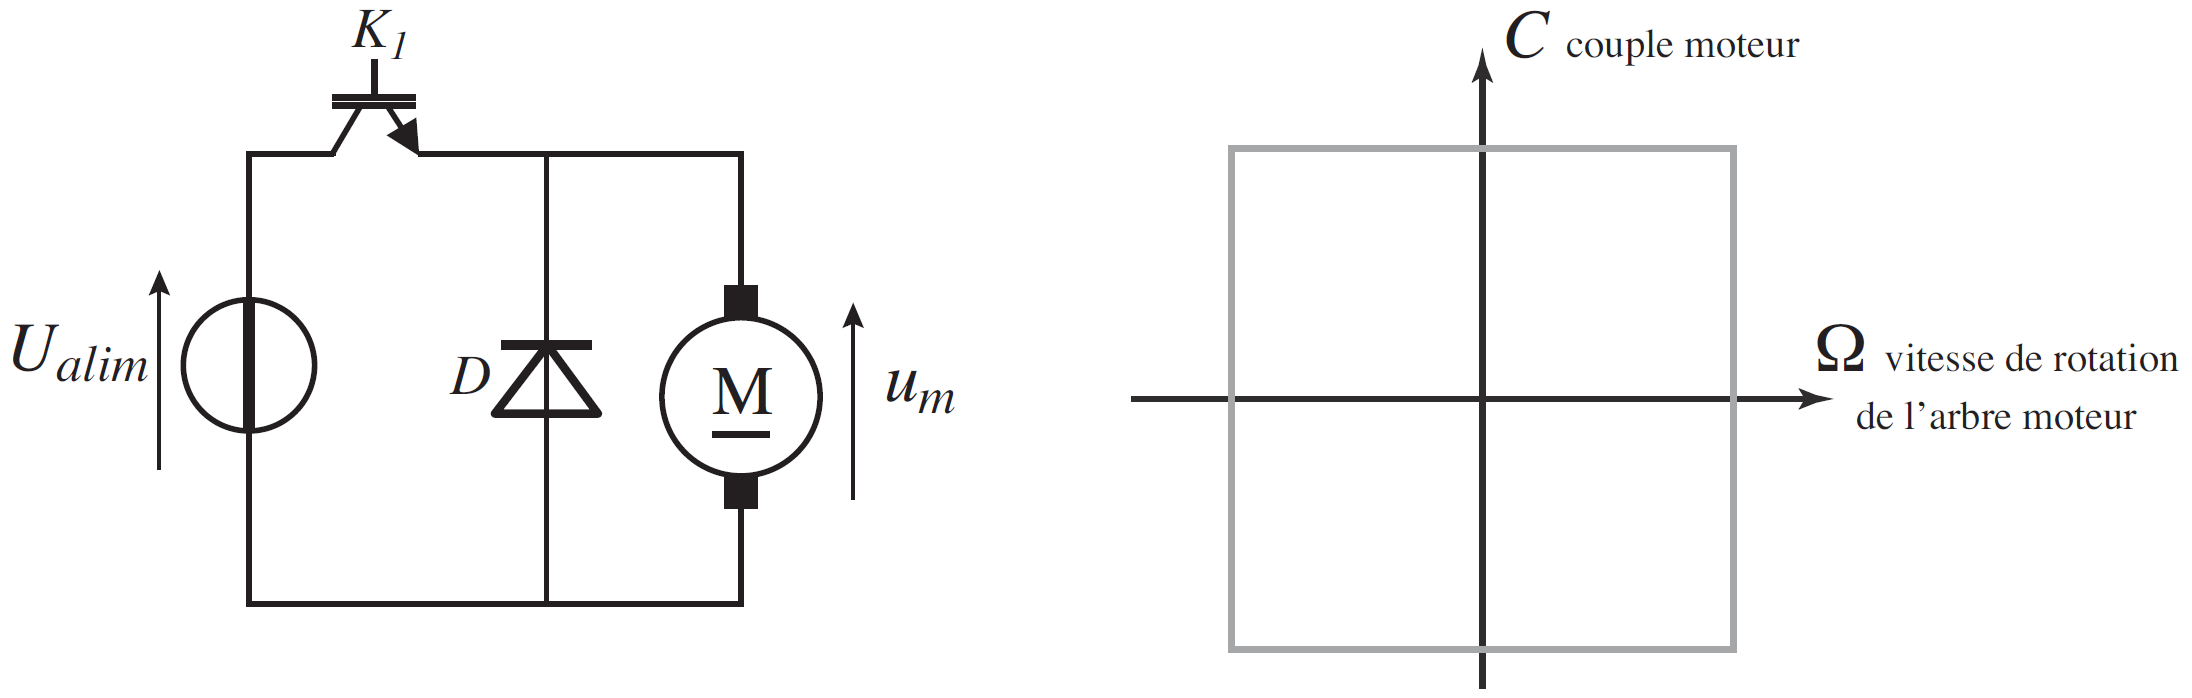
\includegraphics[width=0.9\linewidth]{img/td02_10}
\end{center}}{Le transistor IGBT et la diode sont des composants unidirectionnels en courant donc ce hacheur ne permet qu'un seul sens de courant dans le moteur.

\begin{center}
 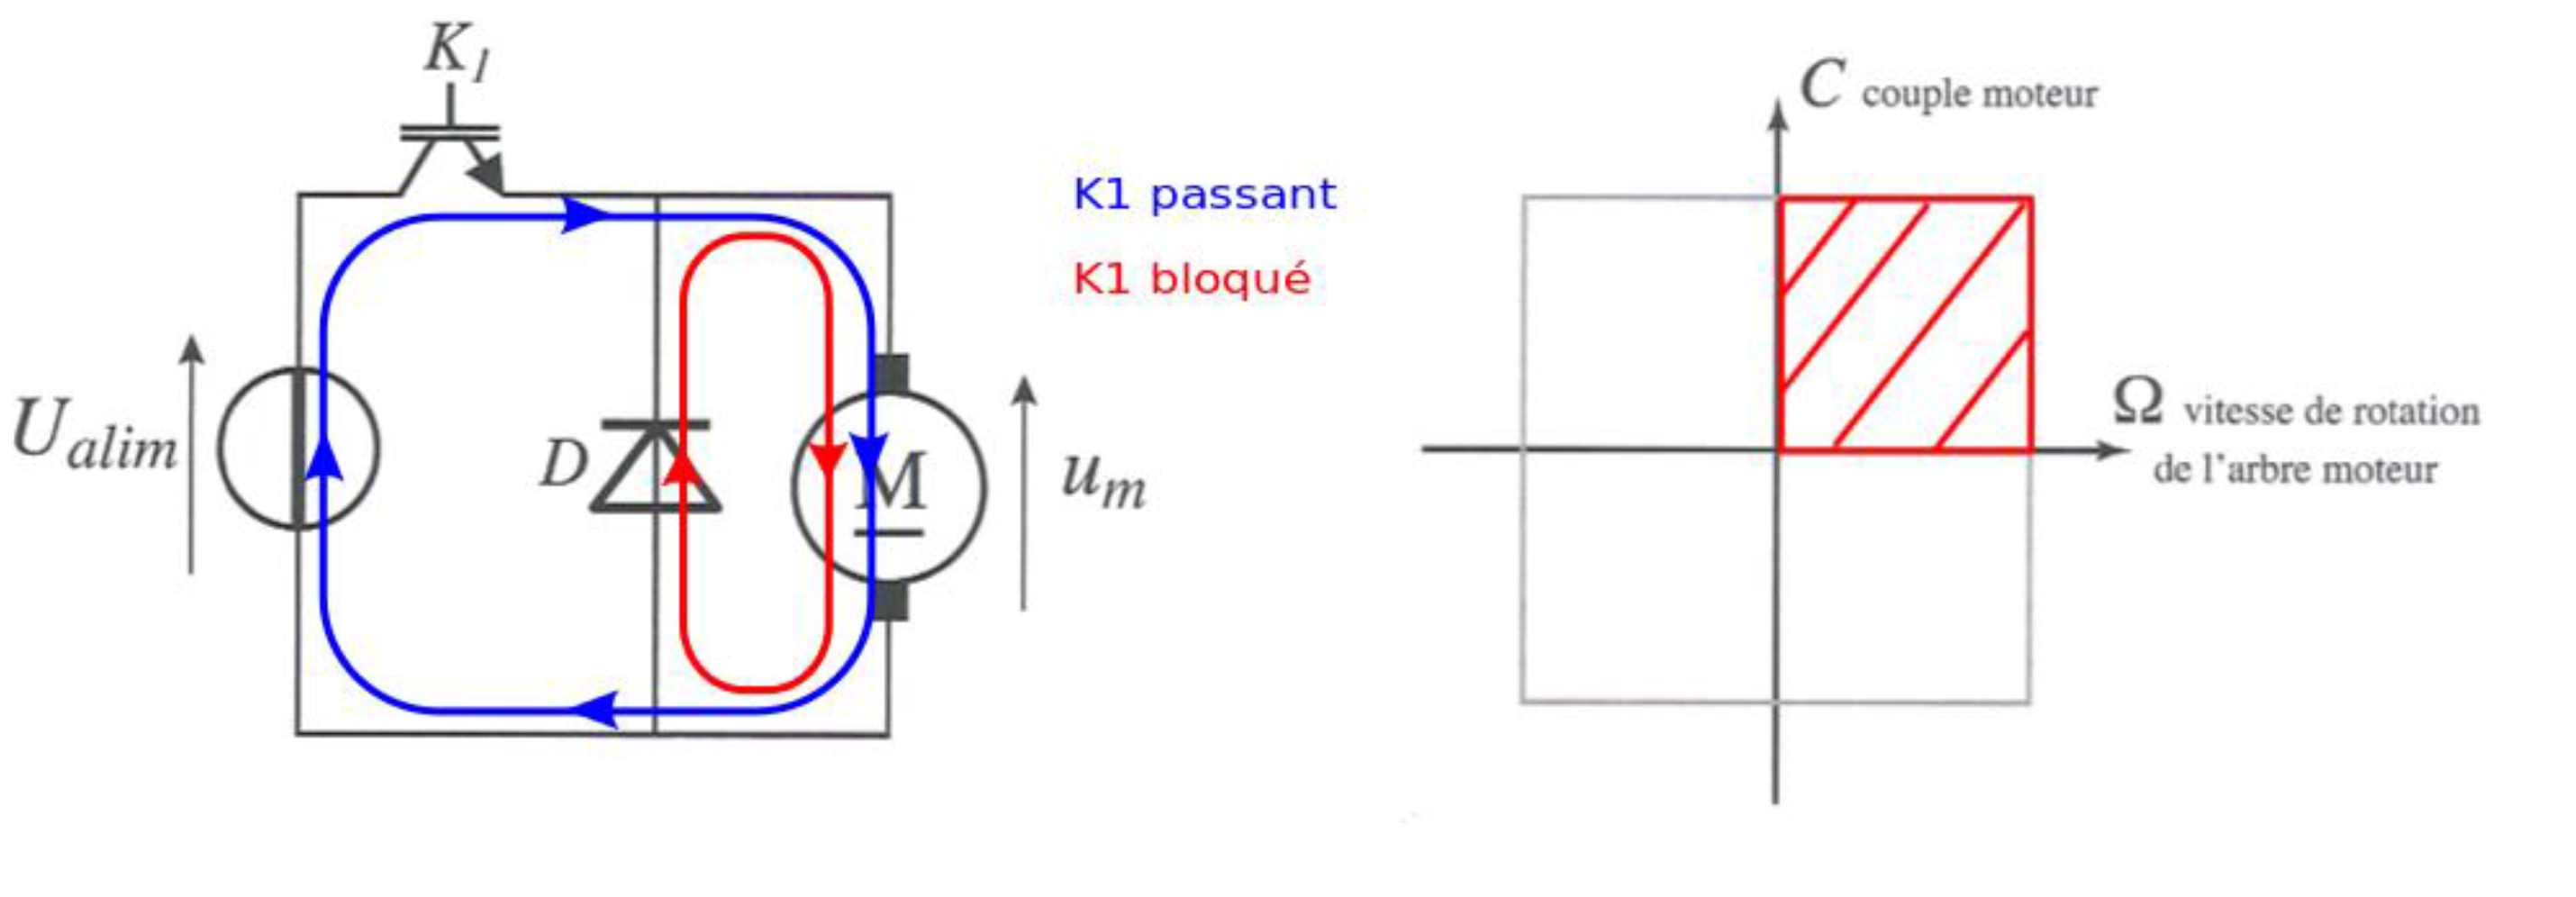
\includegraphics[width=0.9\linewidth]{img/td02_14}
\end{center}}

\reponse{3}{}{Le hacheur proposé est irréversible en tension et ne permet pas d'inverser la tension de commande du moteur. Le moteur ne peut donc pas tourner dans le sens inverse.}

\reponse{3}{\begin{center}
 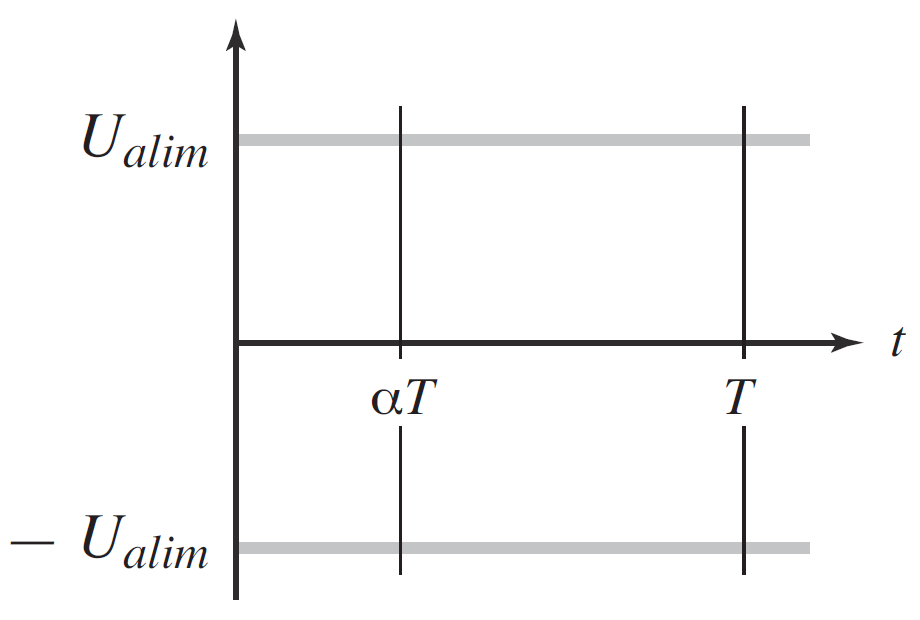
\includegraphics[width=0.5\linewidth]{img/td02_11}
\end{center}}{\begin{center}
 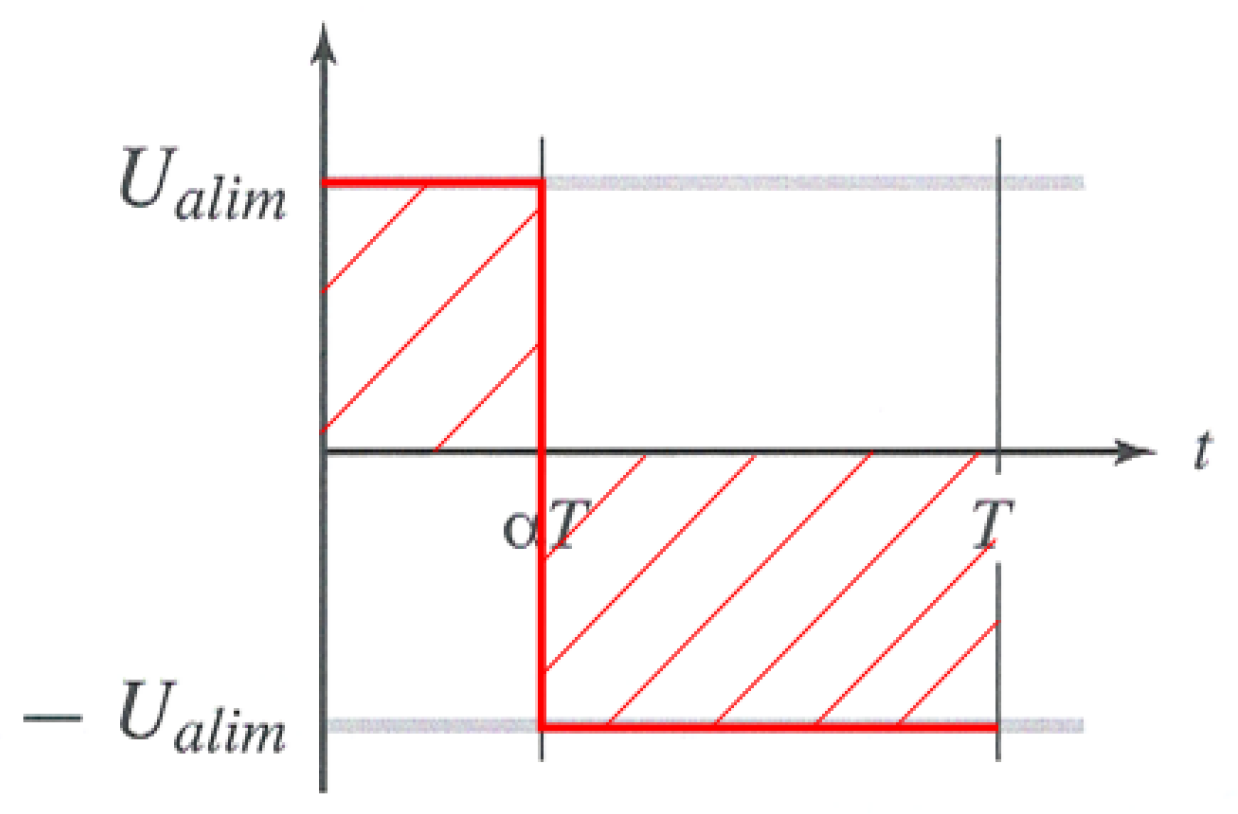
\includegraphics[width=0.5\linewidth]{img/td02_15}
\end{center}

$<u_m>=\frac{\alpha.T.U_{alim}-U_{alim}.(T-\alpha.T)}{T}=U_{alim}.(2.\alpha-1)$

Comme $\alpha\in[0,1]$, on a : $-U_{alim}<u_m<U_{alim}$

$<u_m>$ peut changer de signe, cette plage est donc compatible avec les deux sens de rotation.}

\reponse{4}{\begin{center}
 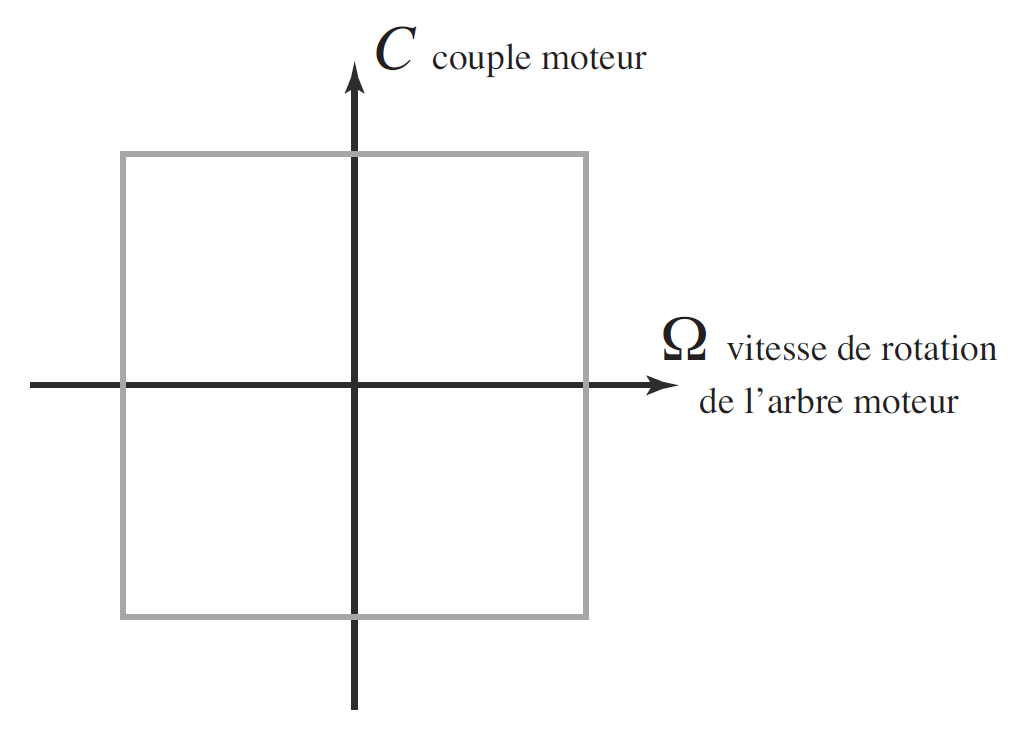
\includegraphics[width=0.4\linewidth]{img/td02_12}
\end{center}}{\begin{center}
 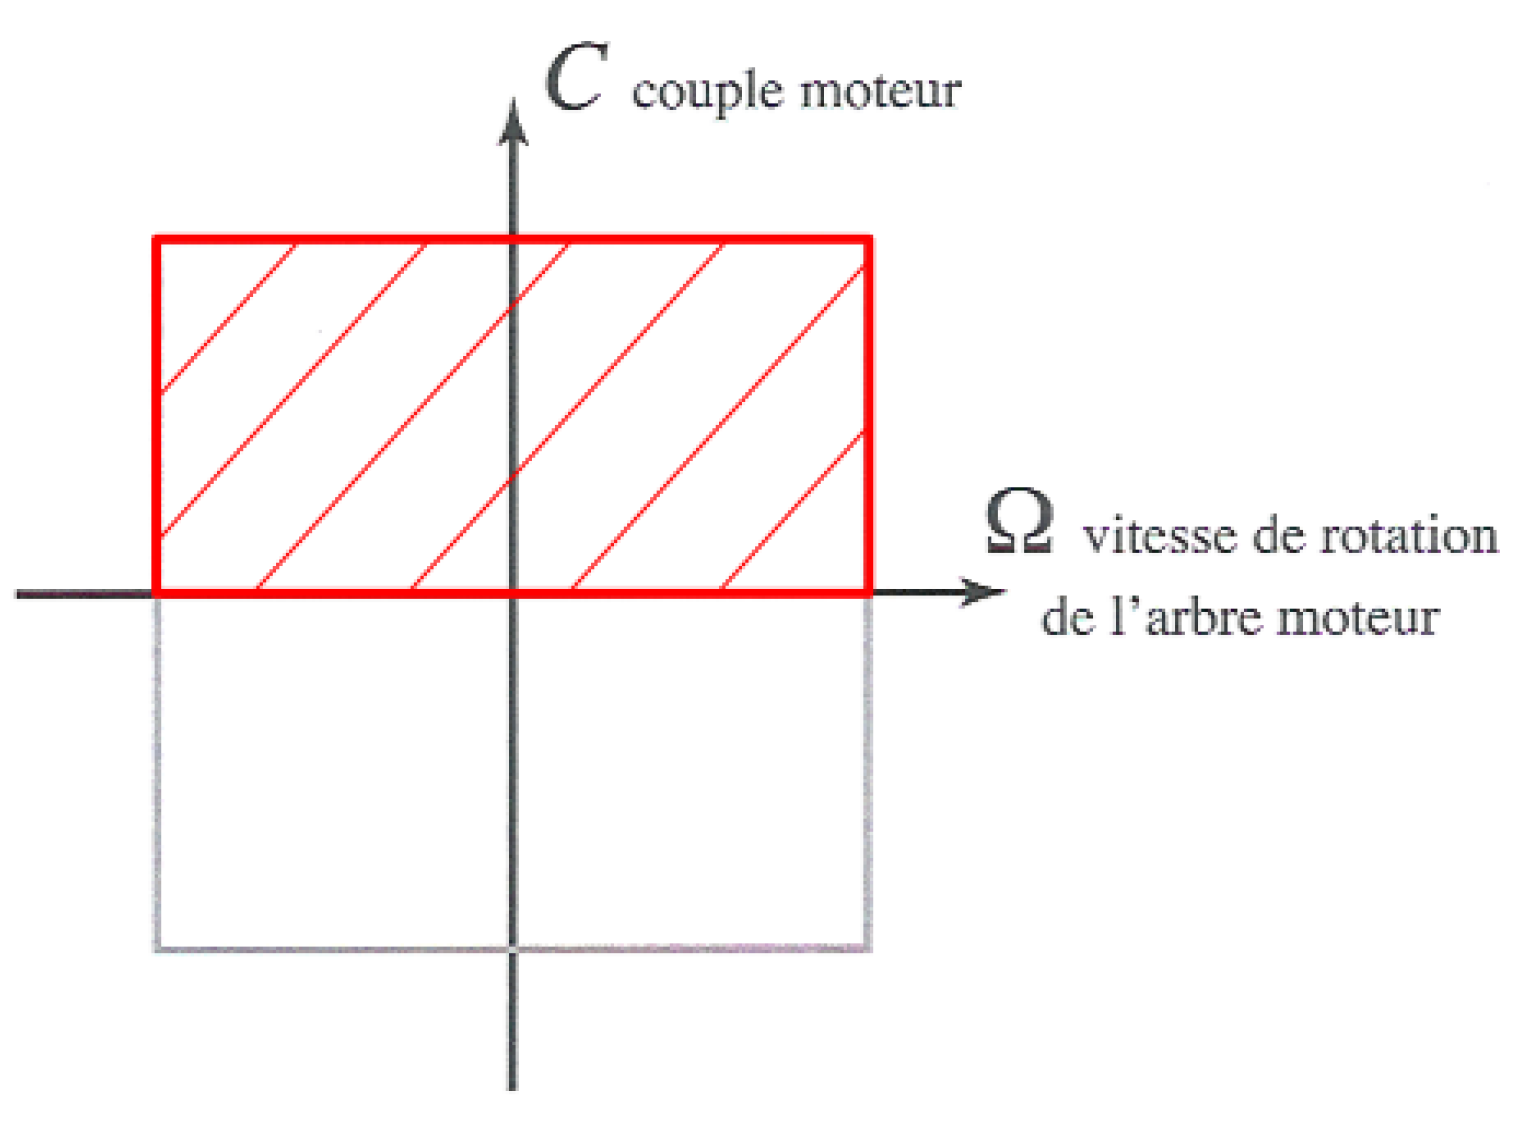
\includegraphics[width=0.4\linewidth]{img/td02_16}
\end{center}

Ce hacheur est réversible en tension et permet d'inverser le sens de rotation du moteur (montée et descente). Par contre, il ne permet de freiner le plateau pendant la phase de descente puisqu'il est irréversible en courant.}

\reponse{4}{}{$2.C_m.\omega_{m1}(t)=m_s.g.v_a(t)$, donc $2.K_i.i_m.\omega_{m1}(t)=m_s.g.\frac{-R_m.R_p}{R_r}.\omega_{m1}(t)$

Donc, $|i_m|=\frac{m_s.g.R_m.R_p}{2.K_i.R_r}=\frac{78.10.20.38.10^{-3}}{2.0,12.30}=78A.$}

\reponse{4}{}{$U_{alim}=e_b+R.i+L.\frac{di}{dt}$}

\reponse{4}{}{$\frac{di}{dt}=(\frac{U_{alim}-e_m}{R}-i).\frac{R}{L}$

Solution sans second membre: $i_g(t)=k.e^{-\frac{t}{\tau_e}}$, avec $\tau_e=\frac{L}{R}$

Solution particulière: $i_p(t)=\frac{U_{alim}-e_m}{R}$

$i_mt)=\frac{U_{alim}-e_m}{R}.(1-e^{-\frac{t}{\tau_e}})+i_0.e^{-\frac{t}{\tau_e}}$}

\reponse{4}{\begin{center}
 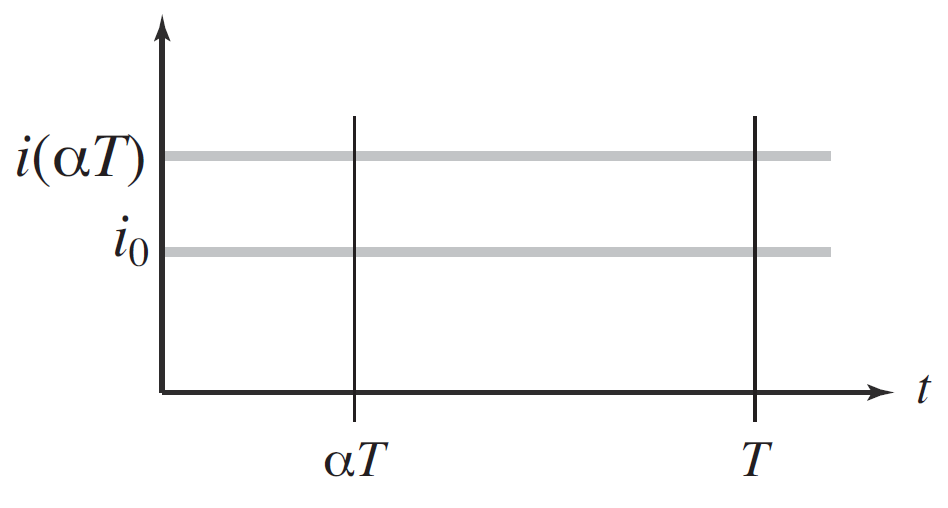
\includegraphics[width=0.6\linewidth]{img/td02_13}
\end{center}}{En faisant un développement limité et en prenant t proche de 0, on obtient:

$i_m(t)=\frac{U_{alim}-e_m}{L}.t+i_0.(1-\frac{t}{\tau_e})$

Et si $t=\alpha.T$ et $T<<\tau_e$, $i(\alpha.T)=\frac{U_{alim}-e_m}{L}.\alpha.T+i_0$.

\begin{center}
 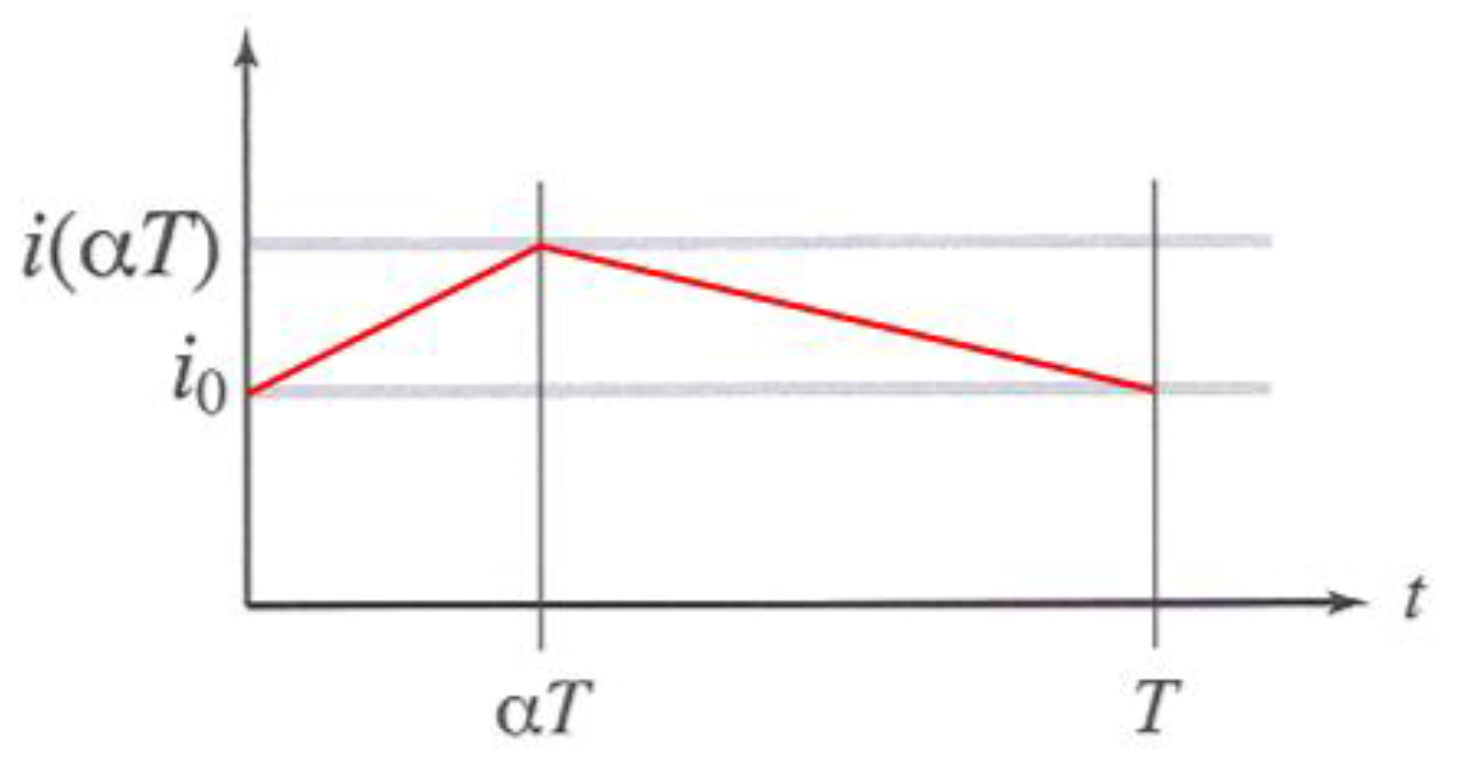
\includegraphics[width=0.6\linewidth]{img/td02_17}
\end{center}}

\reponse{4}{}{Toujours dans les mêmes conditions, on détermine l'augmentation de courant $\Delta_i$ défini par :

$\Delta_i=i(\alpha.T)-i_0=\frac{U_{alim}-e_m}{L}.\alpha.T$}

\reponse{4}{}{$\alpha \in [0,1]$, donc $\Delta_i<\frac{U_{alim}-e_m}{R}.\frac{T}{\tau_e}$

Afin de ne pas perturber le comportement mécanique du moteur, on impose : $\Delta_i\simeq\frac{i_0}{100}$.

On a donc: $\frac{T}{\tau_e}=\frac{R}{U_{alim}-e_m}.\frac{i_0}{100}$

Donc, $\frac{T}{\tau_e}\simeq\frac{2.0,78}{48-36}\simeq\frac{0,4}{3}\simeq 0,13$.}

\reponse{0}{\begin{reponsedoc}[H]
  \centering
  
\includegraphics[width=\linewidth]{img/DR04.png}
  \caption{Schéma-blocs du moteur}
  \label{DR4}
\end{reponsedoc}
}{
% Figure DR4 schéma-blocs
\begin{reponsedoc}[H]
  \centering
   \def\svgwidth{\linewidth}
   \input{img/DR04_cor.pdf_tex}
   \caption{Schéma-blocs du moteur}
  \label{DR4}
\end{reponsedoc}}

\reponse{4}{}{On isole l'ensemble $S$ en équilibre et à l'horizontale ($\alpha$ petit), on effectue le bilan des actions mécaniques extérieures :

\begin{itemize}
  \item Force de la chaîne gauche en $C_g$ : $Y_g\,\vec{y}_0$
  \item Force de la chaîne droite en $C_d$ : $Y_d\,\vec{y}_0$
  \item Poids en $G_S$ : $-m_s g\,\vec{y}_0$
\end{itemize}

Théorème de la résultante statique projeté sur $\vec{y}_0$ :
$Y_g + Y_d - m_s g = 0$

Théorème du moment statique en $C_g$ projeté sur $\vec{z}_0$ :
$0 + Y_d\bigl(L + 2R_p\bigr) - m_s g\!\left(R_p + \dfrac{L}{2} + x_{G_S}\right) = 0$

\[
  Y_d = m_s g\,\frac{R_p + \dfrac{L}{2} + x_{G_S}}{L + 2R_p}
\]

$Y_d = m_s g\!\left(\frac{1}{2} + \frac{x_{G_S}}{L + 2R_p}\right)$

$Y_g = m_s g - Y_d = m_s g\!\left(\frac{1}{2} - \frac{x_{G_S}}{L + 2R_p}\right)$}

\reponse{4}{}{Pour le moteur droit : en supposant le système poulie-courroie parfait, avec les mêmes rayons en entrée et en sortie, on retrouve le même couple en sortie du système poulie-courroie $C_r^d$ exercé sur le pignon droit.

$C_r^d$ est le couple exercée par le poids sur l'axe moteur, donc le couple exercée
sur le pignon est $-C_r^d$.

Le pignon droit est donc en équilibre sous l'action du couple $-C_r^d$ sur l'axe
$(O_d, \vec{z}_0)$, de la force $Y_d\,\vec{y}_0$ en $C_d$ et de l'action du châssis par l'intermédiaire d'une liaison pivot d'axe $(O_d, \vec{z}_0)$. Le théorème de moment statique en $O_d$ projeté sur $\vec{z}_0$ : $-C_r^d + Y_d \cdot R_p + 0 = 0$

$C_r^d = Y_d \cdot R_p = R_p m_s g\!\left(\frac{1}{2} + \frac{x_{G_S}}{L+2R_p}\right)$

$C_r^g = -Y_g \cdot R_p = -R_p m_s g\!\left(\frac{1}{2} - \frac{x_{G_S}}{L+2R_p}\right)$}

\reponse{3}{}{$H_p(p) = \dfrac{R_m + L_m\,p}{K_c}$

$P_p(p)$ en volt (V).}

\reponse{4}{}{Avec $\alpha$ petit :
$\sin\alpha = \dfrac{h_d - h_g}{L} \approx \alpha$
donc $\alpha = \dfrac{1}{L}\cdot(+h_d - h_g)$
ce qui est cohérent avec les signes du schéma-blocs.}

\reponse{4}{}{$h_g(p) = R_p \cdot \dfrac{1}{p} \cdot H_m(p)
        \Bigl(-P_g(p) + U_v(p) - K_{adapt}\,\varepsilon_c(p)\Bigr)$

$h_d(p) = R_p \cdot \dfrac{1}{p} \cdot H_m(p)
        \Bigl(P_d(p) + U_v(p) + K_{adapt}\,\varepsilon_c(p)\Bigr)$}

\reponse{4}{}{Si $P_d(p) = -P_g(p)$ :

\[
  \alpha(p) = \frac{1}{L}\Bigl(h_d(p) - h_g(p)\Bigr)
            = R_p \cdot \frac{1}{p} \cdot H_m(p) \cdot 2K_{adapt} \times \varepsilon_c(p)
            = H_{eq} \times \varepsilon_c(p)
\]

$H_{eq}(p) = \dfrac{2R_p \cdot H_m(p) \cdot K_{adapt}}{p \cdot L}$}

\reponse{4}{}{$H_{BO}(p) = \dfrac{\alpha(p)}{\varepsilon(p)}
       = C_{orr}(p) \times H_{eq}(p)
       = C_{orr}(p) \times \dfrac{2R_p \cdot H_m(p) \cdot K_{adapt}}{p \cdot L}$

$H_m(p)$ est d'ordre 2, donc si $C_{orr}(p) = 1$, $H_{BO}(p)$ est d'ordre 3 et de classe 1.}

\reponse{2}{\begin{reponsedoc}[H]
  \centering
  
\includegraphics[width=0.85\linewidth]{img/DR06.png}
  \caption{Réponse temporelle du système non corrigée en boucle fermée}
  \label{DR6}
\end{reponsedoc}
}{
% Figure DR6 Réponse temporelle
\begin{reponsedoc}[H]
  \centering
   \def\svgwidth{0.85\linewidth}
   \input{img/DR06_cor.pdf_tex}
  \caption{Réponse temporelle du système non corrigée en boucle fermée}
  \label{DR6}
\end{reponsedoc}

Erreur statique : $\varepsilon_s = 0^\circ$ -- exigence 1.3.1.5 respectée

Premier dépassement : $D_{1\%} = \dfrac{0{,}5}{5} = 10\%$ -- exigence 1.3.1.4 respectée de justesse

Temps de réponse à 5\% : $t_{5\%} = 0,7 - 0{,}2 = 0{,}5\,\text{s} > 0{,}1\,\text{s}$ -- Exigence 1.3.1.2 n'est pas respectée}

\reponse{1}{\begin{reponsedoc}[H]
  \centering
  
\includegraphics[width=0.85\linewidth]{img/DR07.png}
  \caption{Diagramme de Bode temporelle du système non corrigée en boucle fermée}
  \label{DR7}
\end{reponsedoc}
}{
% Figure DR7 Diagramme de Bode
\begin{reponsedoc}[H]
  \centering
   \def\svgwidth{0.85\linewidth}
   \input{img/DR07_cor.pdf_tex}
  \caption{Diagramme de Bode du système non corrigée en boucle fermée}
  \label{DR7}
\end{reponsedoc}

D'après l'énoncé $\tau_2 > \tau_1$ donc $\omega_{c2} = \dfrac{1}{\tau_2} < \omega_{c1} = \dfrac{1}{\tau_1}$

$\omega_{c2} = 10\,\text{rad\,s}^{-1}$ donne $\tau_2 = 0{,}1\,\text{s}$

$\omega_{c1} = 3000\,\text{rad\,s}^{-1}$ donne

$\tau_1 = \frac{1}{3000}\,\text{s} = 3{,}3 \times 10^{-4}\,\text{s} = 0{,}33\,\text{ms}$}

%\reponse{4}{}{L'exigence 1.3.1.6 stipule que les perturbations ne doivent pas influencer la précision
%à long terme. Le correcteur Proportionnel Intégral (PI) permet d'ajouter une intégration avant
%la perturbation, et ainsi de rejeter les perturbations de type échelon. Mais le schéma-blocs
%de la figure~20 qui est utilisé pour la simulation du DR5 ne présente pas de perturbation !
%
%Mais ce correcteur va nécessairement faire diminuer la marge de phase quel que soit le réglage, alors que cette dernière n'était déjà pas bonne.
%
%La rapidité peut être améliorée en compensant le pôle dominant s'il y a suffisamment
%de stabilité, mais avec cet unique correcteur PI, ça ne sera pas le cas.
%
%Utiliser uniquement un correcteur PI ne semble pas adapté ! Il faut également améliorer la marge de phase.}
%
%\reponse{4}{}{Le pôle dominant correspond à la constante de temps la plus grande (la plus lente),
%on choisit donc :
%
%$T_i = \tau_2 = 0{,}1\,\text{s}$
%
%$H_{BO}(p) = \dfrac{K_p\,K_{eq}}{\tau_2\,p^2\,(1 + \tau_1\,p)}$}
%
%\reponse{4}{}{Sur le diagramme de Bode de la FTBO avec correcteur PI, la marge de phase est de
%$4^\circ < 75^\circ$ ce qui est très faible. L'ajout du correcteur à avance de phase va permettre de retrouver la stabilité souhaitée en ajoutant une bosse de phase à l'endroit souhaité.}
%
%\reponse{4}{}{En $\omega = 20\,\text{rad\,s}^{-1}$ la marge de phase est de $3^\circ$ sans le correcteur à avance de phase, il faut donc ajouter $\varphi_{max} = 72^\circ$ de phase en $\omega = 20\,\text{rad\,s}^{-1}$
%
%\[
%  \sin(\varphi_{max}) = \frac{a-1}{a+1} \quad\Longrightarrow\quad
%  a = \frac{1 + \sin(\varphi_{max})}{1 - \sin(\varphi_{max})}
%\]
%
%a = 40}
%
%\reponse{4}{}{$\omega_{max} = \dfrac{1}{T_{av}\sqrt{a}} = 20\,\text{rad\,s}^{-1}$ donne
%
%$T_{av} = \frac{1}{\omega_{max}\sqrt{a}} = 8 \times 10^{-3}\,\text{s} = 8\,\text{ms}$}
%
%\reponse{4}{}{D'après la figure~\ref{fig22}, seule la valeur $K_p = 3{,}5$ permet de satisfaire les exigences temporelles suivantes :
%
%\begin{itemize}
%  \item $D_{1\%} = 10\% \leq 10\%$ (exigence 1.3.1.4)
%  \item $t_{5\%} = 0{,}08\,\text{s} < 0{,}1\,\text{s}$ (exigence 1.3.1.2)
%  \item $\varepsilon_s = 0^\circ$ (exigence 1.3.1.5)
%\end{itemize}}

\newif\ifcor
\ifdef{\public}{\corfalse}{\cortrue}

\reponse{0}{}{}

\ifcor
\begin{lstlisting}
import math

def distance(som1 : (int, int), som2 : (int, int)) -> float:
    """
    Renvoie la distance euclidienne entre les deux positions som1 et som2
    """
    dist = 0
    for i in range(len(som1)):
        dist += (som1[i] - som2[i])**2
    return math.sqrt(dist)
\end{lstlisting}
\else
\begin{lstlisting}[escapechar=@]
import math

def distance(som1 : (int, int), som2 : (int, int)) -> float:
    """
    Renvoie la distance euclidienne entre les deux positions som1 et som2
    """
   	@~@
	@~@
	@~@
	@~@
\end{lstlisting}
\fi

\reponse{0}{}{}

\ifcor
\begin{lstlisting}
def voisin_dispo(G : dict, sommet : (int, int),
                 pos_indispo : {(int, int) : str}) -> [(int, int)]:
    """
    G : graphe sous forme de liste d'adjacence.
    sommet : position courante du robot (au temps t).
    pos_indispo : ensemble des positions indisponibles au temps (t+1).
    """
    return [l for l in G[sommet] if l not in pos_indispo]
\end{lstlisting}

Cette forme de liste par compréhension est proposée dans les diverses syntaxes en
Python en début de document réponse et un exemple était proposé dans la fonction
\texttt{trajet} du document réponse à la question Q37 pour créer la liste
\texttt{voisin\_possible}.
\else
\begin{lstlisting}[escapechar=@]
def voisin_dispo(G : dict, sommet : (int, int),
                 pos_indispo : {(int, int) : str}) -> [(int, int)]:
    """
    G : graphe sous forme de liste d'adjacence.
    sommet : position courante du robot (au temps t).
    pos_indispo : ensemble des positions indisponibles au temps (t+1).
    """
   	@~@
	@~@
	@~@
    return 
\end{lstlisting}
\fi

\reponse{0}{}{}

\ifcor
\begin{lstlisting}
def voisin_suivant(ens_voisin : [(int, int)], Sarr : (int, int)) -> (int, int):
    """
    Renvoie la position la plus proche de la position Sarr (au sens de la
    distance euclidienne) parmi les positions contenues dans la liste ens_voisin
    """
    dist_min = math.inf
    suivant = (None, None)
    for voisin in ens_voisin:
        if distance(voisin, Sarr) < dist_min:
            dist_min = distance(voisin, Sarr)
            suivant = voisin
    return suivant
\end{lstlisting}
\else
\begin{lstlisting}[escapechar=@]
def voisin_suivant(ens_voisin : [(int, int)], Sarr : (int, int)) -> (int, int):
    """
    Renvoie la position la plus proche de la position Sarr (au sens de la
    distance euclidienne) parmi les positions contenues dans la liste ens_voisin
    """
	@~@
	@~@
	@~@
	@~@
	@~@
	@~@
	@~@
	@~@
    return suivant
\end{lstlisting}
\fi

\reponse{0}{}{}


\ifcor
\begin{lstlisting}
def trajet(G : dict, tmax : int, Sdep : (int, int), Sarr : (int, int))
    -> [(int, int)]:
    """
    G : Graphe sous forme de liste d'adjacence.
    Sdep : position de depart.
    Sarr : position d'arrivee.
    tmax : temps maximum pour effectuer le trajet.
    Renvoie le chemin entre Sdep et Sarr en choisissant comme
    position suivante la plus proche de Sarr parmi les
    positions voisines non encore atteintes.
    Si le temps de parcours du chemin depasse tmax,
    il n'y a pas de chemin (on renvoie une liste vide)
    """
    chemin = [Sdep]  # debut du chemin en Sdep
    for t in range(tmax + 1):
        if chemin[-1] == Sarr:               # a completer
            return chemin
        # calcul de l'ensemble des positions accessibles a t+1
        pos_indispo = position_skypod(t + 1)             # a completer
        voisin_disponible = voisin_dispo(G, chemin[-1], pos_indispo)  # a completer
        voisin_possible = [v for v in voisin_disponible if v not in chemin]
        # Si position(s) accessible(s) ==> la plus proche de Sarr
        if len(voisin_possible) > 0:
            chemin.append(voisin_suivant(voisin_possible, Sarr))  # a completer
    return []
\end{lstlisting}
\else
\begin{lstlisting}[escapechar=@]
def trajet(G : dict, tmax : int, Sdep : (int, int), Sarr : (int, int))
    -> [(int, int)]:
    """
    G : Graphe sous forme de liste d'adjacence.
    Sdep : position de depart.
    Sarr : position d'arrivee.
    tmax : temps maximum pour effectuer le trajet.
    Renvoie le chemin entre Sdep et Sarr en choisissant comme
    position suivante la plus proche de Sarr parmi les
    positions voisines non encore atteintes.
    Si le temps de parcours du chemin depasse tmax,
    il n'y a pas de chemin (on renvoie une liste vide)
    """
    chemin = [Sdep]  # debut du chemin en Sdep
    for t in range(tmax + 1):
        if                                              # a completer
            return chemin
        # calcul de l'ensemble des positions accessibles a t+1
                                                        # a completer
                                                        # a completer
        voisin_possible = [v for v in voisin_disponible if v not in chemin]
        # Si position(s) accessible(s) ==> la plus proche de Sarr
        if len(voisin_possible) > 0:
                                                        # a completer
    return []
\end{lstlisting}
\fi

%\reponse{4}{}{$m$ : degré maximal d'un sommet, $n$ : ordre du graphe
%
%Dans le pire cas, la boucle \texttt{for} est exécutée $t_{max} + 1$ fois, dans cette boucle on trouve :
%
%\begin{itemize}
%  \item La fonction \texttt{position\_skypod} de complexité constante
%  \item La fonction \texttt{voisin\_dispo} est de complexité $m \times n$ (on remplit une liste de $n$ éléments en réalisant pour chacun un test \texttt{in} de complexité linéaire $m$)
%  \item La création de la liste \texttt{voisin\_possible} est de complexité au pire de $m \times t_{max}$ (on parcourt les \texttt{voisins\_disponibles} ($\leq m$) et on vérifie qu'il n'est pas dans \texttt{chemin} ($\leq t_{max} + 1$))
%  \item La fonction \texttt{voisin\_suivant} est de complexité linéaire $m$ (une boucle \texttt{for} parcourue au maximum $m$ fois qui appelle la fonction \texttt{distance} de complexité linéaire)
%\end{itemize}
%
%Le nombre d'opérations est donc de l'ordre de :
%
%\[
%  (t_{max}+1) \times \bigl(cst_1 + m \times n \times cst_2
%  + m \times t_{max} \times cst_3 + m \times cst_4\bigr)
%\]
%
%La fonction \texttt{trajet} est donc de complexité au pire de cas :
%$t_{max} \times m \times \max(t_{max}, n)$
%
%Si on considère que le nombre de place indisponible est faible devant l'ordre du graphe $n$, dans la formule précédente, on peut assimiler $n$ à une constante, ainsi :
%
%La fonction \texttt{trajet} est donc de complexité au pire de cas :
%$m \times t_{max}^2$}

\reponse{4}{\begin{reponsedoc}[H]
  \centering
  
\includegraphics[width=0.45\linewidth]{img/DR08.png}
  \caption{Chemins possibles de $(0,0)$ à $(2,2)$}
  \label{DR8}
\end{reponsedoc}
}{
% Figure chemins
\begin{reponsedoc}[H]
  \centering
  
\includegraphics[width=0.45\linewidth]{img/DR08_cor.png}
  \caption{Chemins possibles de $(0,0)$ à $(2,2)$}
  \label{DR8}
\end{reponsedoc}

Le chemin parcouru est représenté en vert avec deux possibilités au démarrage.

On constate que la solution n'est pas optimale, les chemin violet est plus court.}

%\reponse{4}{}{}
%\ifcor
%\begin{lstlisting}
%def temps_acces_position(G : dict, tmax : int, Sdep : (int, int))
%    -> {(int, int) : float}:
%    """  # a completer
%    G : Graphe sous forme de liste d'adjacence.
%    tmax : temps maximum pour effectuer le trajet.
%    Sdep : position de depart.
%    Renvoie un dictionnaire des temps minimum pour atteindre chaque sommet depuis Sdep
%    """
%    # temps d'acces initiaux infinis
%    temps_visite = {i : float("int") for i in G}
%
%    # gestion des sommets a visiter
%    file = [Sdep]
%
%    for t in range(tmax + 1):
%        nbre_sommet = len(file)  # ne pas visiter 2 fois un sommet a t
%        while nbre_sommet > 0:
%            som = file.pop()            # som : nouvelle position courante
%            nbre_sommet -= 1
%            if t < temps_visite[som]:   # temps pour atteindre som
%                temps_visite[som] = t
%
%            presence_voisin_non_visite = False
%            for voisin in G[som]:
%                # voisin non encore atteint
%                if temps_visite[voisin] > t :
%                    # et atteignable a t + 1
%                    if voisin not in position_skypod(t+1):
%                        # evite les doublons dans file
%                        if voisin not in file :
%                            file.insert(0, voisin)
%                    else:
%                        presence_voisin_non_visite = True
%                # re-insertion des sommets ayant au moins un voisin
%                # non encore atteint et non atteignable a t + 1
%                if presence_voisin_non_visite and som not in file:
%                    file.insert(0, som)
%    return temps_visite
%\end{lstlisting}
%\fi
%
%\reponse{4}{}{La position $(1,2)$ n'étant pas atteignable pour $t = 3$, elle sera atteinte au temps
%suivant.
%
%% Figure DR8
%\begin{figure}[H]
%  \centering
%  
\includegraphics[width=0.75\linewidth]{img/DR08.png}
%  \caption{Graphe avec temps d'accès minimum complété -- DR8}
%  \label{fig:DR8}
%\end{figure}}
%
%\reponse{4}{}{La fonction \texttt{temps\_accès\_position} reprend le principe de l'algorithme de
%Dijkstra pour le parcours de graphe.
%
%La différence réside dans le fait que l'algorithme de Dijkstra s'utilise sur des graphes pondérés pour déterminer le plus court chemin, alors que pour cet algorithme la « pondération » (temps d'accès entre 2 sommets voisins) est variable dans le temps, car les sommets ne sont pas tous accessibles à chaque instant.}
%
%\reponse{4}{}{Pour trouver le trajet entre \texttt{Sdep} et \texttt{Sarr}, après avoir calculé les temps d'accès minimum avec la fonction \texttt{temps\_accès\_position}, on part du sommet \texttt{Sarr} et on parcourt le graphe en suivant les voisins de proche en proche en choisissant celui qui a le temps d'accès minimum à chaque fois.}
%
%
%% -----------------------------------------------------------
%%  DR5
%% -----------------------------------------------------------
%\newpage
%\begin{center}
%  \textbf{img/DR5 -- Réponses fréquentielle (BO) et temporelle (BF), système non corrigé ($C_{orr}(p) = 1$)}
%
%  \textbf{Q25 et Q26.} Vérification des exigences et tracé asymptotique
%\end{center}
%
%\begin{figure}[H]
%  \centering
%  
\includegraphics[width=\linewidth]{img/DR04.png}
%  \caption{Diagrammes de Bode de la fonction de transfert en boucle ouverte non corrigée.}
%  \label{DR5}
%\end{figure}
%
%\begin{center}
%\renewcommand{\arraystretch}{1.4}
%\begin{tabular}{|l|p{10cm}|}
%  \hline
%  \textbf{Vérification exigences} & \\
%  \hline
%  & \\ & \\ & \\ & \\ & \\
%  \hline
%\end{tabular}
%\end{center}
%
%% -----------------------------------------------------------
%%  Suite DR5 (réponse temporelle) + DR6
%% -----------------------------------------------------------
%\newpage
%
%\begin{figure}[H]
%  \centering
%  
\includegraphics[width=0.55\linewidth]{img/DR06.png}
%  \caption{Réponse temporelle du système non corrigé en boucle fermée}
%  \label{DR6}
%\end{figure}
%
%\begin{center}
%\renewcommand{\arraystretch}{1.4}
%\begin{tabular}{|l|p{10cm}|}
%  \hline
%  \textbf{Vérification exigences} & \\
%  \hline
%  & \\ & \\ & \\ & \\ & \\
%  \hline
%\end{tabular}
%\end{center}
%
%\vspace{0.5cm}
%\begin{center}
%  \textbf{img/DR6 -- Trajet par position la plus proche}
%
%  \textbf{Q37.} Compléter la fonction \texttt{trajet}
%\end{center}
%
%\begin{lstlisting}
%def trajet(G:graph, tmax:int, Sdep:(int,int), Sarr:(int,int)) -> [(int,int)]:
%    """
%    G : graphe sous forme de liste d'adjacence
%    Sdep : position de depart.
%    Sarr : position d'arrivee.
%    tmax : temps maximum pour effectuer le trajet.
%    Renvoie le chemin entre Sdep et Sarr en choisissant comme
%    position suivante la position la plus proche de Sarr parmi les
%    positions voisines non encore atteintes.
%    Si le temps de parcours du chemin depasse tmax,
%    il n'y a pas de chemin (on renvoie une liste vide).
%    """
%    chemin = [Sdep]   # debut du chemin en Sdep
%    for t in range(tmax+1) :
%
%        if                                              :  # a completer
%            return chemin
%
%        # Calcul de l'ensemble des positions accessibles a t+1 :
%
%        pos_indispo = position_skypod(              )   # a completer
%
%        voisin_disponible = voisin_dispo(           )   # a completer
%
%        voisin_possible = [v for v in voisin_disponible if v not in chemin]
%
%        # Si position(s) accessible(s) ==> la plus proche de Sarr
%        if len(voisin_possible) > 0 :
%
%            chemin.append(                          )   # a completer
%    return []
%\end{lstlisting}
%
%% -----------------------------------------------------------
%%  DR7
%% -----------------------------------------------------------
%\newpage
%\begin{center}
%  \textbf{img/DR7 -- Temps d'accès par parcours de graphe}
%
%  \textbf{Q40.} Compléter signature et spécification de la fonction \texttt{temps\_accès\_position}
%\end{center}
%
%\begin{lstlisting}
%def temps_acces_position(G, tmax, Sdep) -> :
%    """ a completer
%
%    """
%    # temps d'acces initiaux infinis :
%    temps_visite = {i : float("inf") for i in G}
%
%    # gestion des sommets a visiter :
%    file = [Sdep]
%
%    for t in range(tmax+1) :
%        nbre_sommet = len(file)   # ne pas visiter 2 fois un sommet a t
%        while nbre_sommet > 0 :
%            som = file.pop()            # som : nouvelle position courante
%            nbre_sommet -= 1
%            if t < temps_visite[som] :  # temps pour atteindre som
%                temps_visite[som] = t
%
%            presence_voisin_non_visite = False
%            for voisin in G[som] :
%                # voisin non encore atteint :
%                if temps_visite[voisin] > t :
%                    # et atteignable a t+1
%                    if voisin not in position_skypod(t+1) :
%                        # evite les doublons dans file
%                        if voisin not in file :
%                            file.insert(0, voisin)
%                    else :
%                        presence_voisin_non_visite = True
%            # re-insertion des sommets ayant au moins un voisin
%            # non encore atteint et non atteignable a t+1
%            if presence_voisin_non_visite and som not in file :
%                file.insert(0, som)
%    return temps_visite
%\end{lstlisting}
%
%% -----------------------------------------------------------
%%  DR8
%% -----------------------------------------------------------
%\newpage
%\begin{center}
%  \textbf{img/DR8 -- Temps d'accès aux positions de l'entrepôt exemple}
%
%  \textbf{Q41.} Compléter les temps d'accès avec \texttt{Sdep=(0,0)}, \texttt{Sarr=(2,2)} et \texttt{tmax=10}.\\
%  La position $(1,2)$ n'est pas atteignable à $t = 2$ et $t = 3$.
%\end{center}
%
%\begin{figure}[H]
%  \centering
%  
\includegraphics[width=0.75\linewidth]{img/DR08.png}
%  \caption{Graphe DR8 -- temps d'accès minimum (à compléter)}
%  \label{DR8}
%\end{figure}

\end{document}
